\documentclass[parskip=full,11pt]{scrartcl}

\usepackage[utf8]{inputenc}
\usepackage[T1]{fontenc}
\usepackage[german]{babel}

\usepackage[yyyymmdd]{datetime} % must be after babel
\renewcommand{\dateseparator}{-} % ISO8601 date format

%%aus der Vorlage übernommen, um identisches Layout zu haben
%%%%%%%%%%%%%%%%%%%%%%%%%%%%%%%%%%%%%%%
%%\usepackage{scrlayer-scrpage}
%%\pagestyle{scrheadings}
\usepackage[sfdefault,light]{roboto}


%%%%%%%%%%%%%%%%%%%%%%%%%%%%%%%%%%%%%%%

\usepackage{fontawesome}

\usepackage{hyperref}
\usepackage{csquotes}
\usepackage{glossaries}
%%Mathpackage
\usepackage{amsmath}

\usepackage[nameinlink]{cleveref}

\usepackage{xcolor}
\usepackage{graphicx}
\graphicspath{ {images/} }
\usepackage{rotating}
\hypersetup{
	pdftitle={Pflichtenheft}
}

\usepackage{pflichtenheft}

\usepackage{float}
\usepackage{enumitem}

% geändert, damit die Verlinkungen in den Testfällen nicht außerhalb des Seitenrands stehen
\usepackage[bottom = 3 cm, top = 3 cm]{geometry}


\usepackage{listings}    
\lstset{
	moredelim=[is][\bfseries]{[*}{*]},
	mathescape,
	numbers=left, 
	numberstyle=\tiny, 
	breaklines=true,
	numbersep=5pt,
	xleftmargin=10pt,
	xrightmargin=5pt,
	tabsize=2} 

\usepackage{tikz}
\usetikzlibrary{positioning,shapes.geometric}

\makeindex
\makeglossaries

% so wird ein Glossareintrag definiert
%\newglossaryentry{computer}{
%	name=computer,
%	description={is a programmable machine that receives input,
%		stores and manipulates data, and provides
%		output in a useful format}
%}

\begin{document}
	\title{Pflichtenheft: Programmanalyse zum Durchklicken}
	\author{Nils Jessen \and Anika Nietzer \and Patrick Petrovic \and Sebastian Rauch \and Michael Schieber}
	
	\maketitle


	%note: don't split this document up with include{...}

\section{Einleitung}

Moderne Compiler übersetzen nicht nur Quellcode, sondern bieten auch die Möglichkeit, Optimierungen durchzuführen. 
Einige dieser Optimierungen basieren auf Datenflussanalysen des Quellcodes bzw. eines Zwischencodes.
Um das Verständnis für auf Datenflussanalyse basierende Optimierungen zu erleichtern, soll hier ein Werkzeug entwickelt werden, welches ausgewählte Datenflussanalysen visualisiert.

\subsection{Kontrollflussgraph}
Das Konzept des Kontrollflussgraphen (CFG) ist zentral für Datenflussanalysen und wird deshalb im Folgenden kurz erklärt.
Ein CFG zu einem Programm (oder einer Funktion / Methode) ist ein Graph, dessen Knoten genau die Grundblöcke des Programms sind.
Ein Grundblock $B$ ist eine maximal lange Folge von Instruktionen, sodass der Kontrollfluss $B$ an höchstens einer Stelle betreten und an höchstens einer Stelle verlassen kann.
Es gibt also im Programm keine Sprünge, deren Ziel nicht Anfang eines Grundblockes ist.
Außerdem stehen Sprungbefehle höchstens am Ende eines Grundblocks.
Zwischen zwei Grundblöcken $B_i$ und $B_j$ gibt es genau dann eine gerichtete Kante $(B_i,B_j)$, wenn der Kontrollfluss unmittelbar von $B_i$ nach $B_j$ wechseln kann.
In diesem Fall heißt $B_i$ Vorgänger von $B_j$ und $B_j$ Nachfolger von $B_i$.
Dies ist z. B. der Fall, wenn am Ende von $B_i$ eine Sprunganweisung steht, deren Ziel der Anfang von $B_j$ ist.

\par

\begin{lstlisting}[frame=single, captionpos=b, caption=Simple Funktion zur Veranschaulichung eines CFG]
int gcd(int a, int b) {
	int tmp;
	while(b != 0) {
		tmp = b;
		b = a % b;
		a = tmp;
	}
	return a;
}
\end{lstlisting}

\par

\begin{figure}[H]
\centering
\begin{tikzpicture}[%
->,
shorten >=2pt,
>=stealth,
node distance=1cm,
noname/.style={%
	ellipse,
	minimum width=5em,
	minimum height=3em,
	draw
}
]
\node [draw] (1) {
\begin{lstlisting}[numbers=none]
int tmp;
\end{lstlisting}
};

\node [draw] (2) [below=of 1] {
\begin{lstlisting}[numbers=none]
if (b != 0)
\end{lstlisting}
};

\node[draw] (3) [below left=of 2]   {
\begin{lstlisting}[numbers=none]
tmp = b;
b = a % b;
a = tmp;
\end{lstlisting}
};

\node[draw] (4) [below right=of 2]   {
\begin{lstlisting}[numbers=none]
return a;
\end{lstlisting}
};

\path (1) edge node {} (2);
\path (2) edge [bend right=20pt] node {} (3);
\path (2) edge node {} (4);
\path (3) edge [bend right=20pt] node {} (2);
\end{tikzpicture}
\caption{CFG zu Listing 1}
\end{figure}

\par

\subsection{Datenflussanalyse}
Eine Datenflussanalyse ist eine statische Code-Analyse, d. h. die Analyse erfolgt lediglich anhand der Struktur des Codes, ohne dass dieser ausgeführt wird. 
Mittels Datenflussanalyse können bestimmte Eigenschaften von Programmen approximiert werden.

\subsubsection{Theoretische Grundlagen}

Datenflussanalysen arbeiten typischerweise auf dem CFG des zu analysierenden Codes.
Im Folgenden werden Grundblöcke als kleinste Einheit betrachtet, auf denen die Analyse operiert.
Für eine Datenflussanalyse benötigt man zunächst eine Grundmenge $D$.
Diese Grundmenge stellt die möglichen Fakten dar, die vor bzw. nach einem Grundblock gelten können.
Zu jedem diskreten Schritt $t$ der Analyse ist jedem Grundblock $B$ ein Eingangszustand $in_B[t] \in D$ und ein Austrittszustand $out_B[t] \in D$ zugeordnet.
Der Eingangszustand von $B$ repräsentiert die bei Eintritt in $B$ geltenden Fakten.
Analog entspricht der Austrittszustand von $B$ den geltenden Fakten bei Verlassen von $B$.

Weiter ist zu jedem Grundblock $B$ eine Überführungsfunktion $f_B:D\to D$ gegeben, die den Austrittszustand in Schritt $t+1$ aus dem Eingangszustand im vorherigen Schritt $t$ berechnet: $out_B[t+1]=f_B(in_B[t])$.
Diese Überführungsfunktion setzt sich aus den Überführungsfunktionen der einzelnen Instruktionen innerhalb dieses Grundblocks zusammen:
Besteht der Grundblock $B$ aus den Instruktionen $I_1,...,I_m$ in dieser Reihenfolge und ist für jede dieser Instruktionen eine Überführungsfunktion $f_{I_k}:D\to D, k\in \{1,..,m\}$ gegeben, so ist $f_B$ als Komposition dieser gegeben: $f_B=f_{I_m}\circ ... \circ f_{I_1}$.
Deshalb genügt es, zu jeder Instruktion eine Überführungsfunktion zu definieren, die die Wirkung dieser Instruktion beschreibt.

Ziel einer Datenflussanalyse ist nun, für jeden Grundblock $B$ ein Faktum $d\in D$ zu finden, das nach $B$ gilt und sich bei obiger Iteration ($out_B[t+1]=f_B(in_B[t])$) nicht mehr ändert.
Dies kann mittels Fixpunktiteration erreicht werden.
Dazu benötigt man zusätzlich zu den Überführungsfunktionen innerhalb der Grundblöcke noch Überführungsfunktionen zwischen den Grundblöcken.
Im Allgemeinen kann ein Grundblock mehrere Vorgänger haben.
Deshalb benötigt man eine Operation, um die Austrittszustände mehrerer Grundblöcke zusammenzuführen.
Diese Operation wird im Folgenden als Join-Operator $\vee :D\times D \to D$ bezeichnet.
Ausgehend davon kann man den Join-Operator für endlich viele $d_1,...,d_n \in D$ definieren: $\bigvee (d_1,..,d_n):=(\bigvee(d_1,...,d_{n-1})) \vee d_n$ für $n \geq 3$ und $\bigvee(d_1,d_2):=d_1 \vee d_2$ (formal kann man noch $\bigvee (d_1):=d_1$ setzen).
Damit kann man Überführungsfunktionen zwischen Grundblöcken definieren: 
Hat der Grundblock $B$ die Vorgänger $P_1,...,P_r$, so ist der Eingangszustand von $B$ im Schritt $t+1$ gegeben als Join der Austrittszustände von $P_1,...,P_r$ im Schritt $t$: $in_B[t+1]=\bigvee(out_{P_1}[t],...,out_{P_r}[t])$.

Bei der Fixpunktiteration wird für $t \in \mathbb{N}$ und jeden Grundblock $B$ der Austrittszustand aus dem Eingangszustand berechnet: $out_B[t+1]=f_B(in_B[t])$. 
Dies wird fortgesetzt, bis erstmals für ein $t_0 \in \mathbb{N}$ für jeden Grundblock $B$ der Austrittszustand konstant bleibt: $out_B[t_0+1]=f_B(in_B[t_0])$.
Damit gilt wegen der Rechtseindeutigkeit der Überführungsfunktionen für die Grundblöcke $f_{B_i}$ sowie der Überführungsfunktionen zwischen den Grundblöcken: $out_B[s+k]=f_B(in_B[s])$ für alle $s,k \in \mathbb{N}$ mit $s \geq t_0$.
Es ändern sich also bei obiger Iteration die Eingangszustände und Ausgangszustände nach Schritt $t_0$ nicht mehr.
Dies bezeichnet man als Fixpunkt des hier beschriebenen iterativen Verfahrens.

Stellt man geeignete Bedingungen an die Grundmenge $D$, die Überführungsfunktion $f_B$ für jeden Grundblock $B$ sowie den Join-Operator $\vee$, so existiert solch ein Fixpunkt notwendigerweise und wird durch obiges Verfahren stets nach endlich vielen Schritten gefunden.


Im Folgenden werden einige Beispiele für Datenflussanalysen und die durch sie approximierten Eigenschaften angegeben.

\subsubsection{Constant Folding}
Beim Constant Folding werden die Werte von Ausdrücken, die bereits bei der Übersetzung ausgewertet werden können, ermittelt.
Eine naheliegende Optimierung ist dann, solche Ausdrücke durch die entsprechenden Werte zu ersetzen.
Damit vermeidet man das Generieren der Instruktionen für diese Ausdrücke. Lediglich eine Instruktion zum Laden einer Konstanten muss dann generiert werden.
\begin{lstlisting}[frame=single, captionpos=b, caption=Beispielcode für Constant-Folding-Analyse]
int x = 2;
int y = -4;
int z = x * x + y * y; 
\end{lstlisting}
Hier steht der Wert von \lstinline{z} bereits bei der Übersetzung fest:
\begin{lstlisting}[numbers=none]
z = 2 * 2 + (-4) * (-4) = 4 + 16 = 20.
\end{lstlisting}
Obiger Code ist also äquivalent zu
\begin{lstlisting}[frame=single, captionpos=b, caption=Mittels Constant-Folding optimierte Version von Listing 2]
int x = 2;
int y = -4;
int z = 20; 
\end{lstlisting}
Hier tauscht man im Vergleich zum ursprünglichen Code zwei Multiplikationen und eine Addition gegen das Laden einer Konstanten ein.

\subsubsection{Constant Bits}
Die Constant-Bits-Analyse ist eng mit dem Constant Folding verwandt. 
Hier interessiert man sich allerdings dafür, welche einzelnen Bits von Variablen konstant sind.
Sind konstante Bits innerhalb von Variablen gefunden, kann diese Information zur Optimierung bestimmter Ausdrücke genutzt werden.

\par

\begin{lstlisting}[frame=single, captionpos=b, caption=Beispielcode für Constant-Bits-Analyse]
int foo(int x) {
	int y = 12 + 8 * x;
	return y % 4 + 2 * x;
} 
\end{lstlisting}

Hier ist \lstinline|y| \textbf{\%} \lstinline|4| immer gleich \lstinline{0}, sodass obiger Code vereinfacht werden kann zu

\par

\begin{lstlisting}[frame=single, captionpos=b, caption=Mittels Constant-Bits-Analyse optimierte Version von Listing 4]
int foo(int x) {
	int y = 12 + 8 * x;
	return 2 * x;
} 
\end{lstlisting}

\subsubsection{Reaching Definitions}
Bei der Reaching-Definitions-Analyse soll für jede Stelle im Programm die Menge der Definitionen (Zuweisungen), die diese Programmstelle erreichen, ermittelt werden.
Eine Definition erreicht eine Stelle genau dann, wenn es einen Pfad im CFG gibt, sodass die Definition auf diesem Pfad vor besagter Stelle auftaucht und nicht wieder überschrieben wird.

\par

\begin{lstlisting}[frame=single, captionpos=b, caption=Beispielcode für Reaching-Definitions-Analyse]
$def_1$: int x = 2;
$def_2$: int y = -4;
$def_3$: x = 2 * y + 10; 
\end{lstlisting}

\par

Betrachtet man das Ende des obigen Codestücks, so sind $def_2$ und $def_3$ Reaching Definitions bezüglich dieser Programmstelle.
$def_1$ erreicht das Ende des Programms nicht, da $def_3$ eine neue Definition von \lstinline{x} gibt, $def_1$ ist danach nicht mehr relevant.

\subsubsection{Taint-Analyse}
In manchen Programmen ist es fatal, wenn Benutzereingaben ohne weitere Überprüfung verarbeitet werden. 
Beispielsweise sollte niemals ein String, der ganz oder teilweise von einem Benutzer stammt, direkt als Anfrage an ein Datenbanksystem weitergegeben werden.
Dies ermöglicht Angriffe wie SQL-Injection, die das Datenbanksystem in ungewollter Weise beeinflussen.
Um diese Angriffe zu vermeiden, sollten alle Anfragen, die aus Benutzereingaben hervorgehen, auf möglicherweise schädliche Effekte untersucht werden.
Das Überprüfen, ob jedes Datenobjekt, das als potentiell schädlich eingestuft wird, vor Weitergabe an kritische Stellen (z. B. Anfrageschnittstelle eines Datenbanksystems) überprüft wurde, kann mittels Taint-Analyse automatisiert geschehen.
Dazu werden Stellen im Programm definiert, die Daten als 'bedenklich' (tainted) markieren.
Weiter gibt es Stellen (z. B. spezielle Methodenaufrufe), die 'bedenkliche' Daten als 'unbedenklich' markieren.
Schließlich gibt es noch Programmstellen, die als kritisch markiert sind.
Ziel der Taint-Analyse ist es nun, sicherzustellen, dass niemals als 'bedenklich' markierte Daten eine als kritisch markierte Programmstelle erreichen.

\subsubsection{Live Variables}
Bei der Live-Variables-Analyse interessiert man sich dafür, ob der Wert einer Variablen vor der nächsten Zuweisung an diese (bzw. vor Programmende, falls keine nächste Zuweisung an diese Variable existiert) benötigt wird. 
Ist dies nicht der Fall, kann diese Zuweisung entfernt werden.

\par

\begin{lstlisting}[frame=single, captionpos=b, caption=Beispielcode für Live-Variables-Analyse]
int incMin(int x, int y) {
	int min;
	if (x < y) {
		min = x;
		x = x + 1;
	} else {
		min = y;
		y = y + 1;
	}
	return min + 1;
}
\end{lstlisting}

\par

Hier haben die beiden Zuweisungen \lstinline{x = x + 1;} und \lstinline{y = y + 1} keinen Effekt und können daher entfernt werden.
Folgender optimierter Code ist also äquivalent:

\par

\begin{lstlisting}[frame=single, captionpos=b, caption=Mittels Live-Variables-Analyse optimierte Version von Listing 7]
int incMin(int x, int y) {
	int min;
	if (x < y) {
		min = x;
	} else {
		min = y;
	}
	return min + 1;
}
\end{lstlisting}

\subsection{Zielsetzung}
Wie bereits zu Anfang formuliert, soll hier ein Werkzeug zur Visualisierung ausgewählter Datenflussanalysen entwickelt werden.
Dazu kann der Benutzer Java-ähnlichen Code (eine Teilmenge der primitiven Datentypen sowie Operatoren und Kontrollflusskonstrukte von Java werden unterstützt) zur Analyse angeben.
Aus diesem Code wird zunächst ein CFG generiert und dem Benutzer angezeigt.
Dann kann der Benutzer die zu visualisierende Datenflussanalyse auswählen.
Es werden mindestens Constant-Folding-, Constant-Bits-, Reaching-Definitions- und Taint-Analyse unterstützt.
Die ausgewählte Datenflussanalyse wird dann ausgeführt und schrittweise anhand des CFG visualisiert.
Zusätzlich hat der Benutzer noch die Möglichkeit, den Fixpunkt der Analyse direkt berechnen zu lassen.

	%note: don't split this document up with include{...}

\section{Kriterien}

\subsection{Muss}

\criterium{Eingabe von Code}{crt:CodeInput}
Eingegebener Java-Code kann zu einem CFG verarbeitet werden.

\criterium{Java-Subset}{crt:minSubset}
Der zu analysierende Code benutzt eine minimale Teilmenge an Java-Operatoren, Kontrollflussstrukturen und Datentypen der Java-Version 1.7. Bei Fehlern wird eine Fehlermeldung ausgegeben.

\criterium{CFG}{crt:CFG}
Generierter Zwischencode wird dem Benutzer in einem CFG angezeigt.

\criterium{Datenflussanalysen}{crt:DFA}
Das Programm kann mehrere Datenflussanalysen ausführen und anhand des CFG visualisieren.
Diese sind:\par
\begin{enumerate}[label=(\alph*)]
\item Constant Folding
\item Reaching Definitions
\item Constant Bits
\item Taint Analysis
\end{enumerate}

\criterium{Anzeigen der Analyse}{crt:ShowAnalysis}
Die Schritte der Datenflussanalysen können dem Benutzer blockweise animiert im CFG angezeigt werden.

\criterium{Fixpunkt}{crt:Fixpunkt}
Das Programm kann den Fixpunkt der Analyse automatisch berechnen.

\newpage

\criterium{Abbruch der Analyse}{crt:AbortAnalysis}
Der Benutzer kann die Analyse abbrechen und zur Code-Eingabe zurückkehren.

\subsection{Kann}

\criteriumOptional{Erweitertes Java-Subset -Priorität 1 (hoch)}{crt:extendedSubset1o}
Das Programm kann Java-Code einlesen und verarbeiten, welcher weitere Operatoren und Konstrukte beinhaltet.

\criteriumOptional{Zeilenangabe bei Fehlermeldungen - Priorität 2 (mittel)}{crt:lineNmbrErrorO}
Entstehen beim Kompilieren des eingelesenen Codes Fehlermeldungen, so wird dem Benutzer angezeigt, in welcher Zeile des Java-Codes der Fehler gemacht wurde.

\criteriumOptional{Breakpoints in Datenflussanalyse - Priorität 2}{crt:BreakpointsO}
Der Benutzer kann Breakpoints in den erstellten CFG setzen. Beim automatisierten Durchlaufen der Analyse stoppt diese am nächsten gesetzten Breakpoint.

\criteriumOptional{Analyse einzelner Zeilen innerhalb der Blöcke - Priorität 1}{crt:lineAnalysisO}
Beim Durchlaufen der Datenflussanalyse erhält der Benutzer zusätzlich zu den In- und Out-Informationen der Blöcke auch In- und Out-Informationen zu den einzelnen Zeilen innerhalb der Blöcke.

\criteriumOptional{Dynamisches Graph-Layout - Priorität 1}{crt:GraphLayoutO}
Der Benutzer hat die Möglichkeit, das zunächst automatisiert erstellte Layout des CFG selbst zu verändern, indem er zoomen und Blöcke bewegen kann.

\criteriumOptional{Einlesen von Code aus .java-Datei und Speichern von Code in .java-Datei - Priorität 3 (niedrig)}{crt:CodeInputExto}
Der Benutzer hat die Möglichkeit, eine .java-Datei in das Programm zu laden, welche
den zu analysierenden Code enthält. Außerdem kann er im Editor des Programms geschriebenen Code in einer .java-Datei speichern.

\newpage

\criteriumOptional{Delay-Optionen zwischen Autoplay-Schritten - Priorität 1}{crt:DelayO}
Der Benutzer kann einstellen, wie lange die einzelnen Schritte im automatisierten
Durchlaufen der Datenflussanalyse angezeigt werden sollen.

\criteriumOptional{Rückwärtsschritte in der Datenflussanalyse - Priorität 1}{crt:backwardsAnalysisO}
Der Benutzer hat die Möglichkeit, in der Datenflussanalyse Schritte zurückzugehen und sich einen vorherigen Analysezustand erneut anzeigen zu lassen.

\criteriumOptional{Auswahlmöglichkeit der Worklistalgorithmen - Priorität 2}{crt:WorklistO}
Der Benutzer kann zwischen verschiedenen Worklistalgorithmen wählen. Diese
entscheiden, in welcher Reihenfolge die Blöcke in der Datenflussanalyse behandelt
werden.

\criteriumOptional{.java-File mit mehreren Funktionen - Priorität 3}{crt:moreFncO}
Der Benutzer kann Java-Code einlesen oder eingeben, welcher mehrere Funktionen
enthält.

\criteriumOptional{\glqq Jump to Action\grqq -Funktion - Priorität 2}{crt:JumpToActionO}
Der Benutzer hat die Möglichkeit den aktuell analysierten Block beziehungsweise die aktuell analysierte Zeile als seinen ausgewählten Block beziehungsweise seine ausgewählte Zeile zu setzen.

\criteriumOptional{Hotkeys für Datenflussanalyse - Priorität 3}{crt:DFAo}
Dem Benutzer steht eine Reihe von Hotkeys zur Navigation durch die
Datenflussanalyse zur Verfügung.

\criteriumOptional{Weitere Datenflussanalysen - Priorität 2}{crt:DFAArtenO}
Der Benutzer kann zur Analyse seines eingegebenen oder eingelesenen Java-Codes
zusätzlich zu den Datenflussanalysen aus M7 aus weiteren Arten der Datenflussanalyse
wählen.

\criteriumOptional{Färbung des CFG - Priorität 1}{crt:HighlightingO}
Die Blöcke des angezeigten CFG im Graph-Panel werden in
Abhängigkeit des aktuellen Analysestandes in verschiedenen Farben eingefärbt.

\criteriumOptional{Exportieren des CFG als Bild-Datei - Priorität 3}{crt:exportPicO}
Der Benutzer hat die Möglichkeit, den aktuell im Graph-Panel angezeigten CFG als Bilddatei zu exportieren. 

\criteriumOptional{Manual Page - Priorität 1}{crt:ManPageO}
Dem Programm liegt eine Manual Page bei, in welcher der Benutzer über die wichtigsten Funktionen des Programms informiert wird.

\criteriumOptional{Fortschrittsanzeige - Priorität 2}{crt:ProgressBarO}
Dem Benutzer wird angezeigt, wie weit die Datenflussanalyse fortgeschritten ist.

\criteriumOptional{Springen zu beliebigem Analysepunkt - Priorität 2}{crt:SliderO}
Der Benutzer kann an einen beliebigen Punkt der Datenflussanalyse springen.

\criteriumOptional{Implementieren einer eigenen Datenflussanalyse - Priorität 3}{crt:OwnAnalyseO}
Der Benutzer kann den CFG mit einer eigenen Datenflussanalyse analysieren.

\newpage
\subsection{Abgrenzung}

\criteriumNot{Kein Tutorial}{crt:noTutorial}
Das Programm erklärt nicht, wie Datenflussanalysen funktionieren oder was ein CFG ist.

\criteriumNot{Keine Optimierung}{crt:noOptimize}
Das Programm ist zur Veranschaulichung von Datenflussanalysen gedacht. Es kann keine Programme optimieren.

\criteriumNot{Funktionalität}{crt:functionality}
Werden folgende Grenzen überschritten, so ist die Funktionalität des Programms nicht mehr garantiert:
\begin{enumerate}[label=(\alph*)]
\item Der CFG hat maximal 10 Blöcke
\item Jeder Block beinhaltet maximal 10 Zeilen Zwischencode
\item Die Datenflussanalyse benötigt maximal 5000 (Zeilen-)Schritte
\item Der eingegebene Java-Code besteht aus maximal 5000 Zeichen
\end{enumerate}
	%note: don't split this document up with include{...}

\section{Produkteinsatz}

... hier der Produkteinsatz ...
	%note: don't split this document up with include{...}

\section{Produktumgebung}

Das Programm ist plattformunabhängig benutzbar.
Eine Java Runtime Environment Version 1.7 ist installiert.

Ein Display mit mindestens 1920x1080 Pixeln steht zur Verfügung.
Ein Intel I5 Prozessor der 4. Generation(Haswell) und 8 GB RAM stehen zur Verfügung.
	%note: don't split this document up with include{...}

\section{Funktionale Anforderungen}

\functionality{Zeilennummerierung}{fnc:LineNumbers}
Im Textfeld für die Eingabe des Codes gibt es eine Zeilennummerierung.

\functionality{Code Eingabe mit Editor}{fnc:CodeInputIntern}
Es gibt ein Textfeld in welches der Benutzer Code eingeben kann, welcher dann zu einem Kontrollflussgraphen (CFG) verarbeitet werden kann.

\functionality{Datei Eingabe}{fnc:CodeInputExt}
Benutzer kann einzulesenden Code aus einer .java Datei laden.

\functionality{Java-Subset}{fnc:minimalSubset}
Das Programm unterstützt ein minimales Subset von Java.
Unterstützt werden:
\begin{enumerate}[label=(\alph*)]
\item Die Arithmetischen Operationen +, -, *, /,
\item die Kontrollflussstrukturen if, else, while,
\item die Vergleichsoperatoren <, >, ==,
\item die Datentypen Integer und Byte,
\item die Zuweisung =.
\end{enumerate}

\functionality{Erweitertes Subset 1}{fnc:extendedSubset1}
Das Programm unterstützt zusätzlich zum minimalen Subset noch:
Die Operatoren \%, <<, >>, |, \&.

\functionality{Erweitertes Subset 2}{fnc:extendedSubset2}
Das Programm unterstützt zusätzlich zum minimalen Subset noch:
For-Schleifen und else-if.

\functionality{Erweitertes Subset 3}{fnc:extendedSubset3}
Das Programm unterstützt zusätzlich zum minimalen Subset noch:
Die Zuweisungen +=, -=, *=, /=, \%=.

\functionality{Syntaxfehler}{fnc:syntaxError}
Enthält der vom Benutzer eingegebene Code Syntaxfehler, so erhält der Benutzer eine Fehlermeldung, welche bezüglich des Informationsgehaltes der Fehlermeldung des Compilers entspricht.

\functionality{Nichtunterstützte Operationen}{fnc:OpsError}
Der Benutzer bekommt eine Fehlermeldung, wenn in der zu analysierenden Funktion Operationen und Kontrollflusskonstrukten vorhanden sind welche nicht dem definierten Subset von Java entsprechen. Die Fehlermeldung weißt auf das unterstütze Java-Subset hin.

\functionality{Anzeigen des Kontrollflussgraphen (CFG)}{fnc:showCFGf}
Die GUI hat kann den aus dem Java-Code erstellten Graphen in einem Zwischencode anzeigen. Dieser Graph ist in einem Panel dargestellt.

\functionality{Interaktion mit dem Kontrollflussgraphen 1}{fnc:interactCFG1f}
Der Benutzer kann mit der GUI des CFG interagieren, um Breakpoints zu setzen.

\functionality{Interaktion mit dem Kontrollflussgraphen 2}{fnc:interactCFG2f}
Der Benutzer kann mit der GUI des CFG interagieren, um zu scrollen und zu zoomen.

\functionality{Interaktion mit dem Kontrollflussgraphen 3}{fnc:interactCFG3f}
Der Benutzer kann mit der GUI des CFG interagieren, um Blöcke, beziehungsweise Zeilen auszuwählen.

\functionality{Auswahl der Analysearten}{fnc:pickAnalysis}
Der Benutzer kann zwischen allen implementierten Analysearten auswählen und sie auf den Graph anwenden.

\functionality{Blockweise durchlaufen der Analyse}{fnc:blockAnalysis}
Der Benutzer kann die Analyse blockweise durchlaufen. Dafür stehen ihm Buttons zur Verfügung.\par
\faFastForward\ : Springt einen Block weiter.\par
\faFastBackward\ : Springt einen Block zurück.

\functionality{Zeilenweise durchlaufen der Analyse}{fnc:lineAnalysis}
Der Benutzer kann die Analyse zeilenweise durchlaufen. Dafür stehen ihm Buttons zur Verfügung.\par
\faForward\ : springt eine Zeile weiter.\par
\faBackward\ : springt eine Zeile zurück.

\functionality{Abbrechen der Analyse}{fnc:stopAnalysisf}
Der Benutzer kann eine laufende Analyse abbrechen, um neuen Code analysieren zu lassen.

\functionality{Automatisches durchlaufen der Analyse}{fnc:automaticAnalysis}
Der Benutzer kann den \faPlay\ Button betätigen, um die Analyse automatisch bis zum Fixpunkt Durchzulaufen.

\functionality{Automatisches durchlaufen bis Breakpoint}{fnc:breakAnalysisf}
Die Analyse kann den \faPlay\ Button betätigen, um automatisch bis zu einem gesetzten Breakpoint laufen.

\functionality{Worklistalgorithmen}{fnc:worklistNaive}
Das Programm kann zur Fixpunktanalyse den naiven Worklistalgorithmus anwenden.

\functionality{Erweiterte Worklistalgorithmen}{fnc:moreWorklist}
Der Nutzer kann zwischen verschiedenen Worklistalgorithmen wählen. Diese
entscheiden, in welcher Reihenfolge die Knoten in der Datenflussanalyse behandelt
werden. Es stehen folgende Algorithmen zur Auswahl:
\begin{enumerate}[label=(\alph*)]
\item \textbf{Naiv} \par
Von oben nach unten, von links nach rechts werden all Knoten in der Reihenfolge in
die Worklist geschrieben, in welcher sie „entdeckt“ werden und dann in dieser
Reihenfolge abgearbeitet.
\item \textbf{Random} \par
Die Blöcke werden wie naiven Worklistalgorithmus auf die Worklist geschrieben. Am Ende der Abarbeitung jedes Knotens in der Analyse wird ein
zufälliger neuer dieser Blöcke gewählt und behandelt.
\item \textbf{Efficient} \par
Die Reihenfolge der Abarbeitung der Blöcke wird optimiert, indem beispielsweise
zuerst innere Schleifen durchlaufen werden, bis ein lokaler Fixpunkt gefunden wurde, bevor die äußere Schleife weiter analysiert wird.
\end{enumerate}

\functionality{Code speichern}{fnc:saveCode}
Der Benutzer kann den Inhalt des Textfeldes zur Codeeingabe in einer .java Datei abspeichern.

\functionality{Hotkeys}{fnc:Hotkeys}
Dem Benutzer stehen Hotkeys zur Verfügung mit Hilfe derer er die Datenflussanalyse steuern kann.

\functionality{Optisches Hervorheben der Blöcke}{fnc:Highlights}
Je nach Status werden die Blöcke im Kontrollflussgraphen farbig hervorgehoben.
\begin{enumerate}[label=(\alph*)]
\item Es gibt die Zustände:
\item Noch nicht besucht.
\item Auf der Worklist.
\item Gerade ausgewählt.
\item Bereits besucht und nicht mehr auf der Worklist.
\end{enumerate}

\functionality{Eingangs- und Ausgangszustand von Blöcken}{fnc:inOutBlockf}
Dem Benutzer werden Eingangs- und Ausgangszustand des ausgewählten Blocks in einem GUI-Element angezeigt.

\functionality{Eingans- und Ausgangszustand von Zeilen}{fnc:inOutLinef}
Dem Benutzer werden Eingangs- und Ausgangszustand der ausgewählten Zeile in einem GUI-Element angezeigt.

\functionality{Graphen exportieren}{fnc:exportAsPicf}
Der Benutzer kann von allen Schritten der Analyse ein Bild des Graphen abspeichern.

\functionality{Ungespeicherte Änderungen}{fnc:unsavedChangesf}
Gibt es ungespeicherte Änderungen im Editor, wenn der Benutzer das Programm schließen möchte, so wird er gefragt, ob er diese speichern möchte.
Falls der Benutzer eine neue .java Datei öffnen möchte und ungespeicherte Änderungen vorliegen, so wird der Benutzer gewarnt, dass diese Änderungen verfallen.

\functionality{Jump to Action}{fnc:jumpToActionf}
Der Benutzer kann mit Hilfe eines Buttons das automatische Springen zum aktiven Block, beziehungsweise zur aktiven Zeile aktivieren. Dieses bleibt so lange aktiv bis er den Button erneut betätigt.

\functionality{Manual Page}{fnc:ManPagef}
Dem Programm liegt eine Manual Page bei, in welcher der Benutzer über die wichtigsten Funktionen des Programms informiert wird.
	%note: don't split this document up with include{...}

\section{Nichtfunktionale Anforderungen}

\nonFunctionality{Benutzeroberfläche reagiert zu jedem Zeitpunkt}{nfc:reactivity}

Die Benutzeroberfläche reagiert in jedem Zustand des Programms (also auch während der Berechnung der Datenflussanalyse) innerhalb von einer Sekunde auf Eingaben des Benutzers.

\nonFunctionality{Visuelles Feedback}{nfc:feedback}

Nach Betätigung eines Buttons erhält der Benutzer innerhalb von einer Sekunde visuelles Feedback.

\nonFunctionality{Konsistenz zwischen Code und CFG}{nfc:consistency}

Der eingelesene oder eingegebene Java-Code ist zu jedem Zeitpunkt konsistent zum angezeigten CFG, sofern ein CFG angezeigt wird.

\nonFunctionality{Aussagekräftige Fehlermeldungen}{nfc:errors}

Java-Kenntnisse und ein Verständnis für das Konzept von Datenflussanalysen vorausgesetzt, enthalten die durch das Programm angezeigten Fehlermeldungen sowohl zum eingegebenen Java-Code als auch zu den Einstellungen des Programms in Kombination mit der Manual Page ausreichend Informationen, dass die Ursache des jeweiligen Fehlers präzise festgestellt werden kann.

\nonFunctionality{Garantierte Funktionalität}{nfc:guarantees}

Die Funktionalität der Analyse ist garantiert, solange keine der folgenden Grenzen überschritten wird:
\begin{enumerate}[label=(\alph*)]
\item Der CFG hat maximal 10 Blöcke
\item Jeder Block beinhaltet maximal 10 Zwischencode-Zeilen
\item Die Datenflussanalyse benötigt maximal 5000 (Zeilen-)Schritte
\item Der eingegebene Java-Code besteht aus maximal 5000 Zeichen
\end{enumerate}

Die übersichtliche Darstellung des CFG ist gewährleistet, solange zusätzlich zu den oben genannten Grenzen keine der folgenden Grenzen überschritten wird:
\begin{enumerate}[label=(\alph*)]
\item Der CFG hat insgesamt maximal 7 Blöcke
\item Jeder Block beinhaltet maximal 5 Zwischencode-Zeilen
\end{enumerate}

\newpage

\nonFunctionality{Skalierbarkeit der GUI}{nfc:scalability}

Die GUI ist beliebig skalierbar für Auflösungen größer oder gleich der geforderten Mindestauflösung (siehe Produktumgebung).

\nonFunctionality{Äquivalenz von Einlesen und Eingabe}{nfc:equivalence}

Das Programm behandelt direkt eingegebenen Java-Code vollständig äquivalent zu aus einer .java-Datei eingelesenem Java-Code.

	\section{Tests (Allgemein)}

\test{Interaktion mit dem Programm unabhängig von der aktuellen Analyse}{tst:general}
\tests{fnc:LineNumbers}
\tests{fnc:unsavedChangesf}
\tests{fnc:ManPagef}


\teststep{Der Benutzer hat das Programm noch nicht geöffnet.}
{Der Benutzer klickt auf die entsprechende Ausführungsdatei.}
{Das Programm öffnet sich mit den definierten GUI-Eigenschaften.}

\teststep{Der Benutzer befindet sich an einer beliebigen Stelle des Arbeitsflusses.}
{Der Benutzer ändert die Fenstergröße.}
{Der Inhalt des Fensters wird dynamisch angepasst.}

\teststep{[opt] Der Benutzer befindet sich an einer beliebigen Stelle des Arbeitsflusses.}
{Der Benutzer möchte sich über die wichtigsten Funktionen des Programms informieren.}
{Eine Manual Page ist dem Programm beigelegt, die diese Information enthält.}

\teststep{[opt] Der Benutzer befindet sich an einer beliebigen Stelle des Arbeitsflusses.}
{Er klickt rechts auf einen Pfeil/Button, der die Leiste verkleinern soll.}
{Die rechte Leiste wird ausgeblendet und das Graph-Panel wird um den frei gewordenen Platz erweitert.}

\teststep{[opt] Der Benutzer befindet sich an einer beliebigen Stelle des Arbeitsflusses. Im Editor steht Java-Code, der bisher nicht gespeichert wurde.}
{Der Benutzer klickt auf einen Button, der zum schließen des Programms führt.}
{In einem Fenster wird darauf hingewiesen, dass die Änderungen bei Fortsetzung der Aktion verloren gehen und eine Möglichkeit, den Vorgang abzubrechen, wird gegeben.}



\test{Schreiben und speichern von Code für die Analyse}{test:writeSave }
\tests{fnc:CodeInputIntern}
\tests{fnc:saveCode}

\teststep{Der Benutzer befindet sich nicht in einer aktuellen Analyse und hat noch keinen Java-Code für die Analyse zur Verfügung.}
{Der Benutzer tippt den zu analysierenden Code in ein Textfeld.}
{Dieser Code steht für die Analyse zur Verfügung.}

\teststep{[opt] Ein Code-Stück ist im Textfeld dargestellt.}
{\glqq Save... \grqq\ wird geklickt.}
{Ein Fenster öffnet sich, in dem der Benutzer den Namen der Datei und ihren Speicherort auswählen kann. Durch klicken des \glqq Speicher\grqq -Buttons wird die Datei gespeichert und das Fenster schließt sich wieder.}


\test{Importieren von Code für die Analyse}{test:import}
\tests{fnc:CodeInputExt}


\teststep{[opt] Der Benutzer befindet sich nicht in einer aktuellen Analyse und hat noch keinen Java-Code für die Analyse zur Verfügung.}
{\glqq Open...\grqq\ wird geklickt.}
{Ein File-Chooser öffnet sich und der Benutzer kann in seinem Dateisystem nach der zu verwendenden Java-Datei suchen.}

\teststep{[opt] Der Benutzer befindet sich nicht in einer aktuellen Analyse und hat nicht gespeicherten Code in seinem Editor.}
{\glqq Open...\grqq\ wird geklickt.}
{In einem Fenster wird darauf hingewiesen, dass die Änderungen bei Fortsetzung der Aktion verloren gehen und eine Möglichkeit, den Vorgang abzubrechen wird gegeben. Wenn kein Abbruch erfolgt, öffnet sich der File-Chooser.}

\teststep{[opt] Der File-Chooser ist geöffnet.}
{Der Benutzer öffnet ein Directory, das keine Datei mit der Endung .java enthält.}
{Es werden keine Dateien angezeigt.}

\teststep{[opt] Der File-Chooser ist geöffnet.}
{Eine Java-Datei wird zum Importieren ausgewählt.}
{Der File-Chooser schließt sich und die Datei wird im Editor angezeigt.}


\test{Auswahl der Datenflussanalyse}{tst:anaopt}
\tests{fnc:pickAnalysis}
\tests{fnc:worklistNaive}
\tests{fnc:moreWorklist}

\teststep{Der Benutzer befindet sich nicht in einer aktuellen Analyse.}
{Der Benutzer wählt eine Datenflussanalyse aus.}
{Diese Datenflussanalyse wird bei dem nächsten Aufruf von \glqq Start Analysis \grqq\ verwendet.}

\teststep{[opt] Der Benutzer befindet sich nicht in einer aktuellen Analyse.}
{Der Benutzer wählt einen Worklist-Algorithmus aus.}
{Dieser Worklist-Algorithmus wird beim nächsten Aufruf von \glqq Start Analysis \grqq\ verwendet.}

\newpage

\test{Erstellen eines CFG}{tst:creategraph}
\tests{fnc:syntaxError}
\tests{fnc:OpsError}
\tests{fnc:showCFGf}
\tests{fnc:Highlights}
\tests{fnc:moreFncf}
\tests{fnc:minimalSubset}
\tests{fnc:extendedSubset1}

\teststep{[opt] Ein Code-Stück, welches nur gültige Java-Syntax aus dem unterstützten Java-Subset enthält, ist im Textfeld dargestellt. Es besteht aus nur einer Methode.}
{\glqq Start Analysis \grqq\ wird geklickt}
{Der CFG wird im Graph-Panel dargestellt und die Animation kann jetzt mit \faStepForward\ oder \faPlay\ gestartet werden. Eine Änderung der Datenflussanalyse oder des Codes ist nur durch Abbruch der Analyse mit \faStop\  möglich.}

\teststep{Ein Code-Stück ist im Textfeld dargestellt, das entweder nicht gültige Java-Syntax enthält, oder solchen Java-Code, dessen übersetzter Zwischencode nicht identisch zum Zwischencode eines Teils des unterstützten Java-Subsets ist.}
{\glqq Start Analysis \grqq\ wird geklickt.}
{Der CFG wird nicht erstellt, eine aussagekräftige Fehlermeldung wird ausgegeben, in der der Java-Error oder ein Hinweis auf das unterstützte Java-Subset gegeben wird.}

\teststep{[opt] Ein Code-Stück ist im Textfeld dargestellt, das gültige Java-Syntax aus dem unterstützten Java-Subset enthält. Es besteht aus mehreren Methoden.}
{\glqq Start Analysis \grqq\ wird geklickt.}
{Ein Fenster öffnet sich, in dem die Methode ausgewählt werden kann, für welche der CFG erstellt und die Analyse durchgeführt werden soll.}


\test{Interaktion mit dem CFG}{tst:intcfg}
\tests{fnc:interactCFG2f}
\tests{fnc:interactCFG2bf}
\tests{fnc:interactCFG3f}

\teststep{[opt] Ein CFG wurde erstellt.}
{Der Benutzer scrollt mit dem Mausrad nach oben bzw. unten, während sich der Mauszeiger im Graph-Panel befindet.}
{Der gesamte CFG wird entsprechend skaliert. Falls der CFG nicht vollständig im Graph-Panel angezeigt werden kann, erscheinen Scroll-Leisten.}

\teststep{[opt] Ein CFG wurde erstellt.}
{Der Benutzer verschiebt per \glqq Drag and Drop \grqq einen Block.}
{Der Block verschiebt sich an die entsprechende Stelle und alle Kanten werden entsprechend mitverschoben. Überlappen sich nun 2 Blöcke, befindet sich der Block, welcher zuletzt verschoben wurde, im Vordergrund.}

\newpage

\test{Bildexport}{tst:graph}
\tests{fnc:exportAsPicf}

\teststep{[opt] Ein CFG wurde erstellt.}
{\glqq CFG exportieren \grqq\ wird geklickt.}
{Ein Fenster öffnet sich, in dem der Benutzer wählen kann, ob er den aktuell angezeigten Zwischenschritt oder alle Zwischenschritte speichern möchte und ob diese zeilenweise oder blockweise gespeichert werden. Außerdem kann er hier zwischen der Auflösung \glqq low \grqq\, \glqq standard \grqq\ und  \glqq  high \grqq\ wählen. Nach Bestätigen dieser Eingabe öffnet sich ein File-Explorer, in dem der Name und der Speicherort der Datei festgelegt werden kann. Alle Bilder werden als PNG-Datei gespeichert. Nach Bestätigen dieser Eingabe mit  \glqq Speichern \grqq\ wird das Bild dort abgelegt.}


\test{Abbrechen der Analyse}{tst:aniposs}
\tests{fnc:stopAnalysisf}


\teststep{Der \glqq Start Analysis \grqq\ Button wurde geklickt.}
{Es wird \faStop\ geklickt.}
{Der Benutzer wird gefragt, ob er seine Analyse wirklich abbrechen möchte und wird darüber informiert, dass dieser Schritt den bisherigen CFG löscht. Bei Bestätigung dieser Meldung wird der CFG gelöscht und das Graph-Panel mit den Animations-Buttons ausgegraut. Eine Änderung des Codes und der Datenflussanalyse ist jetzt wieder möglich.}


\test{Animation in Zusammenhang mit der Delay-Auswahl}{tst:delay}
\tests{fnc:interactCFG1f}
\tests{fnc:automaticAnalysis}
\tests{fnc:breakAnalysisf}
\tests{fnc:jumpToActionf}
\tests{fnc:Delayf}

\teststep{Es wurde in der Zeitauswahl 0 Sekunden als Delay ausgewählt und es wurden keine Breakpoints gesetzt.}
{Es wird \faPlay\ geklickt.}
{Der Fixpunkt wird so schnell wie möglich angezeigt, alle Zwischenschritte werden in der Darstellung übersprungen.}

\teststep{[opt] Es wurde in der Zeitauswahl ein von 0 Sekunden verschiedenes Delay ausgewählt, es wurden keine Breakpoints gesetzt.}
{Es wird der Button \faPlay\ geklickt.}
{Die einzelnen Schritte der Analyse werden mit einem zeitlichen Abstand, der dem ausgewählten Delay entspricht, dargestellt. Die Farben der Blöcke ändern sich je nach Zustand zwischen den verschiedenen Schritten. Zusätzlich ändert sich bei jedem Schritt die rechte Leiste, welche \glqq in \grqq\ und \glqq out \grqq\ des aktuellen Schritts, sowie den aktuellen Schritt selbst anzeigt.}

\teststep{[opt] Es wurden Breakpoints innerhalb des CFG gesetzt.}
{Es wird der Button \faPlay\ geklickt.}
{Die Analyse läuft schrittweise mit dem jeweiligen Delay ab, wobei garantiert wird, dass bei jedem Erreichen eines Breakpoints die Analyse automatisch pausiert wird.}

\teststep{[opt] Die Analyse wurde gestartet und der \glqq jump to action \grqq\ Button ist gesetzt.}
{Es wird der Button \faPlay\ geklickt.}
{Bei jedem neuen Analyseschritt, der angezeigt wird, wird der CFG so zentriert, dass der aktuell analysierte Block in der Mitte liegt. Passt der CFG komplett in das Graph-Panel, so wird nichts verändert.}


\test{Animation bei schrittweiser Berechnung}{tst:calcpart}
\tests{fnc:blockAnalysis}
\tests{fnc:lineAnalysis}
\tests{fnc:stopAnalysisf}
\tests{fnc:inOutBlockf}
\tests{fnc:inOutLinef}


\teststep{Der \faPlay\ Button wurde geklickt und es wurde bisher weder der \faStop\ noch der \faPause\ Button geklickt.}
{Der \faPause\ Button wird geklickt.}
{Die Analyse pausiert im aktuellen Zustand.}

\teststep{Die Analyse wurde durchgeführt und befindet sich im Zustand Pause.}
{Der Button \faStepForward\ wird geklickt.}
{Das Graph-Panel zeigt den Zustand der Analyse zu Beginn der nächsten Zeile an. Die Farben der Blöcke ändern sich, sowie auch das \glqq in \grqq\ und \glqq out \grqq\ der rechten Informationsleiste.}

\teststep{[opt] Die Analyse wurde durchgeführt und befindet sich im Zustand Pause.}
{Der Button \faFastForward\ wird geklickt.}
{Das Graph-Panel zeigt den Zustand der Analyse zu Beginn des nächsten Blocks an. Die Farben der Blöcke ändern sich, sowie auch das \glqq in \grqq\ und \glqq out \grqq\ der rechten Informationsleiste.}

\teststep{Die Analyse wurde durchgeführt und befindet sich im Zustand Pause.}
{Es wird der Button \faStepBackward\ geklickt.}
{Es wird der Zustand der Analyse in der vorhergehende Zeile angezeigt. Die Farben der Blöcke und die Informationen in der rechten Leiste zeigen wieder diesen Zustand an. Gibt es keine vorherige Zeile, wird der Startzustand angezeigt.}

\teststep{[opt] Die Analyse wurde durchgeführt und befindet sich im Zustand Pause.}
{Der Button \faFastBackward\ wird geklickt.}
{Es wird der Zustand der Analyse zu Beginn des aktuellen Blocks angezeigt oder der Beginn des letzten Blocks, falls derzeit die erste Zeile eines Blocks dargestellt wird. Gibt es keinen vorherigen Block, wird der Startzustand angezeigt.}

\teststep{Die Analyse wurde durchgeführt und die Darstellung befindet sich eine Zeile vor dem Fixpunkt.}
{Der Button \faStepForward\ oder \faFastForward\ wird geklickt.}
{Es wird der Zustand der Analyse im Fixpunkt angezeigt und es wird eine Meldung gegeben, die über das Erreichen des Fixpunktes informiert.}

\test{Interaktion mit dem CFG während der Analyse}{tst:interaction}
\tests{fnc:inOutBlockf}
\tests{fnc:inOutLinef}
\tests{fnc:Hotkeys}


\teststep{Die Analyse wurde an einer beliebigen Stelle angehalten.}
{Der Benutzer klickt im CFG auf einen bestimmten Block.}
{Der \glqq in \grqq\ und \glqq out \grqq\ State zum aktuellen Analysezeitpunkt des gewählten Blocks wird in der Informationsleiste rechts angezeigt.}

\teststep{Die Analyse wurde an einer beliebigen Stelle angehalten.}
{Der Benutzer klickt im CFG auf eine bestimmte Zeile.}
{Der \glqq in \grqq\ und \glqq out \grqq\ State zum aktuellen Analysezeitpunkt der gewählten Zeile und des zugehörigen Blocks wird in der Informationsleiste rechts angezeigt.}

\teststep{[opt] Der Benutzer befindet sich an einer beliebigen Stelle des Arbeitsflusses.}
{Der Benutzer verwendet einen der definierten Hotkeys.}
{Die entsprechende, hinterlegte Funktion wird ausgeführt.}

\test{Animation durch Verwendung des Sliders}{tst:Slider}
\tests{fnc:ProgressBarf}
\tests{fnc:Sliderf}

\teststep{[opt] Die Analyse wurde an einer beliebigen Stelle angehalten.}
{Der Benutzer bewegt den Slider in eine beliebige Richtung.}
{Die Analyse springt zu dem dadurch bestimmten Punkt.}

\test{Implementierung einer eigenen Datenflussanalyse}{tst:OwnAnalyse}
\tests{fnc:OwnAnalysef}

\teststep{[opt] Der Benutzer befindet sich nicht in einer aktuellen Analyse.}
{Der Benutzer lädt ein Plugin, welches eine andere, funktionierende Datenflussanalyse enthält.}
{Diese Datenflussanalyse kann nun auf den CFG angewendet werden.}
	\section{Tests (Datenflussanalysen)}

Im Folgenden wird die Analyse als Beispiel für den Worklistalgorithmus \glqq Naiv\grqq\ angegeben.
%%Der Fixpunkt bei der Anwendung anderer Algorithmen ist gleich.
In diesem Beispiel wird davon ausgegangen, dass das erweiterte Java-Subset implementiert wurde.
Der CFG wird exemplarisch in Java-Code angegeben und nicht in Zwischencode wie in der implementierten Analyse.
%Hierbei wird angenommen, dass bei einer Verzweigung der linke Pfad bei einer wahren Bedingung und der rechte Pfad bei einer nicht erfüllten Bedingung genommen wird.


\subsection{Constant Folding}

Zu analysierender Code: \par

\begin{lstlisting}[frame=single]
int constFolding(int n) {
	int x = 6;
	int y = 2 * n;
	while (n > 0) {
		y = y - x;
		x = 3 * (x % 4);
		n = n - 1;
	}
	return y;
}
\end{lstlisting}

\par

\begin{figure}[H]

\centering
\begin{tikzpicture}[%
->,
shorten >=2pt,
>=stealth,
node distance=1cm,
noname/.style={%
	ellipse,
	minimum width=5em,
	minimum height=3em,
	draw
}
]

\node [draw] (1) {
\begin{lstlisting}[numbers=none]
In = {$n= \top, x = \perp, y = \perp$}
[*int x = 6;
int y = 2 * n;*]
Out = {$n= \top, x = \perp, y = \perp$}
\end{lstlisting}
};

\node [draw] (2) [below =of 1] {
\begin{lstlisting}[numbers=none]
In = {$n= \top, x = \perp, y = \perp$}
[*if (n > 0)*]
Out = {$n= \top, x = \perp, y = \perp$}
\end{lstlisting}
};

\node[draw] (3) [below left = 5 cm and 1 cm =of 2] {
\begin{lstlisting}[numbers=none]
In = {$n= \top, x = \perp, y = \perp$}
[*return y;*]
Out = {$n= \top, x = \perp, y = \perp$}
\end{lstlisting}
};

\node[draw] (4) [below right = 5 cm and 1 cm =of 2] {
\begin{lstlisting}[numbers=none]
In = {$n= \top, x = \perp, y = \perp$}
[*y = y - x;
x = 3 * (x % 4);
n = n - 1;*]
Out = {$n= \top, x = \perp, y = \perp$}
\end{lstlisting}
};

\path (1) edge node {} (2);
\path (2) edge [bend right=20pt] node {} (3);
\path (2) edge [bend right=20pt] node {} (4);
\path (4) edge [bend right=20pt] node {} (2);
\end{tikzpicture}

\caption{CFG im initialen Zustand der Constant-Folding-Analyse}
\end{figure}

\begin{figure}[H]
\centering
\begin{tikzpicture}[%
->,
shorten >=2pt,
>=stealth,
node distance= 1cm,
noname/.style={%
	ellipse,
	minimum width=5em,
	minimum height=3em,
	draw
}
]

\node [draw] (1) {
\begin{lstlisting}[numbers=none]
In = {$n= \top, x = \perp, y = \perp$}
[*int x = 6;
int y = 2 * n;*]
Out = {$n= \top, x = 6, y = \top$}
\end{lstlisting}
};

\node [draw] (2) [below =of 1] {
\begin{lstlisting}[numbers=none]
In = {$n= \top, x = \perp, y = \perp$}
[*if (n > 0)*]
Out = {$n= \top, x = \perp, y = \perp$}
\end{lstlisting}
};

\node[draw] (3) [below left  = 5 cm and 1 cm =of 2] {
\begin{lstlisting}[numbers=none]
In = {$n= \top, x = \perp, y = \perp$}
[*return y;*]
Out = {$n= \top, x = \perp, y = \perp$}
\end{lstlisting}
};

\node[draw] (4) [below right = 5 cm and 1 cm=of 2] {
\begin{lstlisting}[numbers=none]
In = {$n= \top, x = \perp, y = \perp$}
[*y = y - x;
x = 3 * (x % 4);
n = n - 1;*]
Out = {$n= \top, x = \perp, y = \perp$}
\end{lstlisting}
};

\path (1) edge node {} (2);
\path (2) edge [bend right=20pt] node {} (3);
\path (2) edge [bend right=20pt] node {} (4);
\path (4) edge [bend right=20pt] node {} (2);
\end{tikzpicture}
\caption{CFG nach Abarbeitung des ersten Blocks der Constant-Folding-Analyse}
\end{figure}

\par

\begin{figure}[H]

\centering
\begin{tikzpicture}[%
->,
shorten >=2pt,
>=stealth,
node distance=1cm,
noname/.style={%
	ellipse,
	minimum width=5em,
	minimum height=3em,
	draw
}
]

\node [draw] (1) {
\begin{lstlisting}[numbers=none]
In = {$n= \top, x = \perp, y = \perp$}
[*int x = 6;
int y = 2 * n;*]
Out = {$n= \top, x = 6, y = \top$}
\end{lstlisting}
};

\node [draw] (2) [below =of 1] {
\begin{lstlisting}[numbers=none]
In = {$n= \top, x = 6, y = \top$}
[*if (n > 0)*]
Out = {$n= \top, x = 6, y = \top$}
\end{lstlisting}
};

\node[draw] (3) [below left  = 5 cm and 1 cm=of 2] {
\begin{lstlisting}[numbers=none]
In = {$n= \top, x = 6, y = \top$}
[*return y;*]
Out = {$n= \top, x = 6, y = \top$}
\end{lstlisting}
};

\node[draw] (4) [below right  = 5 cm and 1 cm=of 2] {
\begin{lstlisting}[numbers=none]
In = {$n= \top, x = 6, y = \top$}
[*y = y - x;
x = 3 * (x % 4);
n = n - 1;*]
Out = {$n= \top, x = 6, y = \top$}
\end{lstlisting}
};

\path (1) edge node {} (2);
\path (2) edge [bend right=20pt] node {} (3);
\path (2) edge [bend right=20pt] node {} (4);
\path (4) edge [bend right=20pt] node {} (2);
\end{tikzpicture}
\caption{CFG im Fixpunkt der Constant-Folding-Analyse}
\end{figure}

\newpage

\subsection{Constant Bits}

Zu analysierender Code: \par

\begin{lstlisting}[frame=single]
int constantBits(int p) {
	int x = 8 * p;
	int y = 0;
	if (p > 0) {
		y = x % 2;
	} else {
		y = x % 4;
	}
	return x + y;
}
\end{lstlisting}

\par

\begin{figure}[H]
\centering
\begin{tikzpicture}[%
->,
shorten >=2pt,
>=stealth,
node distance=1cm,
noname/.style={%
ellipse,
minimum width=5em,
minimum height=3em,
draw
}
]
\node [draw] (1) {
\begin{lstlisting}[numbers=none]
In$_1$ = $\{p=\top, x=\perp, y=\perp \}$
[*int x = 8 * p;
int y = 0;*]
Out$_1$ = $\{p=\top, x=\perp, y=\perp \}$
\end{lstlisting}
};

\node [draw] (2) [below=of 1] {
\begin{lstlisting}[numbers=none]
In$_2$ = $\{p=\top, x=\perp, y=\perp \}$
[*if (p > 0)*]
Out$_2$ = $\{p=\top, x=\perp, y=\perp \}$
\end{lstlisting}
};

\node[draw] (3) [below left=1cm and -2cm of 2]   {
\begin{lstlisting}[numbers=none]
In$_3$ = $\{p=\top, x=\perp, y=\perp \}$
[*y = x % 2;*]
Out$_3$ = $\{p=\top, x=\perp, y=\perp \}$
\end{lstlisting}
};

\node[draw] (4) [below right=1cm and -2cm of 2]   {
\begin{lstlisting}[numbers=none]
In$_4$ = $\{p=\top, x=\perp, y=\perp \}$
[*y = x % 4;*]
Out$_4$ = $\{p=\top, x=\perp, y=\perp \}$
\end{lstlisting}
};

\node[draw] (5) [below left=1cm and -2cm of 4]   {
\begin{lstlisting}[numbers=none]
In$_5$ = $\{p=\top, x=\perp, y=\perp \}$
[*return x + y;*]
Out$_5$ = $\{p=\top, x=\perp, y=\perp \}$
\end{lstlisting}
};

\path (1) edge node {} (2);
\path (2) edge node {} (3);
\path (2) edge node {} (4);
\path (3) edge node {} (5);
\path (4) edge node {} (5);

\end{tikzpicture}
\caption{CFG im Initialzustand der Constant-Bits-Analyse}
\end{figure}

\par

\begin{figure}[H]
\centering
\begin{tikzpicture}[%
->,
shorten >=2pt,
>=stealth,
node distance=1cm,
noname/.style={%
ellipse,
minimum width=5em,
minimum height=3em,
draw
}
]
\node [draw] (1) {
\begin{lstlisting}[numbers=none]
In$_1$ = $\{p=\top, x=\perp, y=\perp \}$
[*int x = 8 * p;
int y = 0;*]
Out$_1$ = $\{p=\top, x=(\top,..., \top,0,0,0), y=(0,...,0) \}$
\end{lstlisting}
};

\node [draw] (2) [below=of 1] {
\begin{lstlisting}[numbers=none]
In$_2$ = $\{p=\top, x=(\top,..., \top,0,0,0), y=(0,...,0) \}$
[*if (p > 0)*]
Out$_2$ = $\{p=\top, x=(\top,..., \top,0,0,0), y=(0,...,0) \}$
\end{lstlisting}
};

\node[draw] (3) [below left=1cm and -4cm of 2]   {
\begin{lstlisting}[numbers=none]
In$_3$ = $\{p=\top, x=\perp, y=\perp \}$
[*y = x % 2;*]
Out$_3$ = $\{p=\top, x=\perp, y=\perp \}$
\end{lstlisting}
};

\node[draw] (4) [below right=1cm and -4cm of 2]   {
\begin{lstlisting}[numbers=none]
In$_4$ = $\{p=\top, x=\perp, y=\perp \}$
[*y = x % 4;*]
Out$_4$ = $\{p=\top, x=\perp, y=\perp \}$
\end{lstlisting}
};

\node[draw] (5) [below left=1cm and -2cm of 4]   {
\begin{lstlisting}[numbers=none]
In$_5$ = $\{p=\top, x=\perp, y=\perp \}$
[*return x + y;*]
Out$_5$ = $\{p=\top, x=\perp, y=\perp \}$
\end{lstlisting}
};

\path (1) edge node {} (2);
\path (2) edge node {} (3);
\path (2) edge node {} (4);
\path (3) edge node {} (5);
\path (4) edge node {} (5);

\end{tikzpicture}
\caption{CFG nach 2 Schritten der Constant-Bits-Analyse}
\end{figure}

\par

\begin{figure}[H]
\centering
\begin{tikzpicture}[%
->,
shorten >=2pt,
>=stealth,
node distance=1cm,
noname/.style={%
ellipse,
minimum width=5em,
minimum height=3em,
draw
}
]
\node [draw] (1) {
\begin{lstlisting}[numbers=none]
In$_1$ = $\{p=\top, x=\perp, y=\perp \}$
[*int x = 8 * p;
int y = 0;*]
Out$_1$ = $\{p=\top, x=(\top,..., \top,0,0,0), y=(0,...,0) \}$
\end{lstlisting}
};

\node [draw] (2) [below=0.8 cm of 1] {
\begin{lstlisting}[numbers=none]
In$_2$ = $\{p=\top, x=(\top,..., \top,0,0,0), y=(0,...,0) \}$
[*if (p > 0)*]
Out$_2$ = $\{p=\top, x=(\top,..., \top,0,0,0), y=(0,...,0) \}$
\end{lstlisting}
};

\node[draw] (3) [below left=0.8cm and -4cm of 2]   {
\begin{lstlisting}[numbers=none]
In$_3$ = $\{p=\top, x=(\top,..., \top,0,0,0), y=(0,...,0) \}$
[*y = x % 2;*]
Out$_3$ = $\{p=\top, x=(\top,..., \top,0,0,0), y=(0,...,0) \}$
\end{lstlisting}
};

\node[draw] (4) [below right=0.8cm and -4cm of 3]   {
\begin{lstlisting}[numbers=none]
In$_4$ = $\{p=\top, x=(\top,..., \top,0,0,0), y=(0,...,0) \}$
[*y = x % 4;*]
Out$_4$ = $\{p=\top, x=(\top,..., \top,0,0,0), y=(0,...,0) \}$
\end{lstlisting}
};

\node[draw] (5) [below left=0.8cm and -4cm of 4]   {
\begin{lstlisting}[numbers=none]
In$_5$ = $\{p=\top, x=(\top,..., \top,0,0,0), y=(0,...,0) \}$
[*return x + y;*]
Out$_5$ = $\{p=\top, x=(\top,..., \top,0,0,0), y=(0,...,0) \}$
\end{lstlisting}
};

\path (1) edge node {} (2);
\path (2) edge node {} (3);
\path (2) edge node {} (4);
\path (3) edge node {} (5);
\path (4) edge node {} (5);

\end{tikzpicture}
\caption{CFG im Fixpunkt der Constant-Bits-Analyse}
\end{figure}

\subsection{Reaching Definitions}

Zu analysierender Code: \par

\begin{lstlisting}[frame=single]
int reachingDefs(boolean c) {
	int a, b;
	a = 1;
	b = 2;
	a = 2;
	if (c) {
	  a = 3;
	} else {
	  a = 5;
	  b = 10;
	}
	return b;
}
\end{lstlisting}

\par

\begin{figure}[H]

\centering
\begin{tikzpicture}[%
->,
shorten >=2pt,
>=stealth,
node distance=1cm,
noname/.style={%
	ellipse,
	minimum width=5em,
	minimum height=3em,
	draw
}
]

\node [draw] (1) {
\begin{lstlisting}[numbers=none]
In = {}
[*int a, b;
a = 1;
b = 2;
a = 2;*]
Out = {}
\end{lstlisting}
};

\node [draw] (5) [below = 1 of 1] {
\begin{lstlisting}[numbers=none]
In = {}
[*if (c)*]
Out = {}
\end{lstlisting}
};

\node [draw] (2) [below left = 3.7 cm and 4 cm =of 5] {
\begin{lstlisting}[numbers=none]
In = {}
[*a = 3;*]
Out = {}
\end{lstlisting}
};

\node[draw] (3) [below right = 3.5 cm and 4 cm =of 5] {
\begin{lstlisting}[numbers=none]
In = {}
[*a = 5;
b = 10;*]
Out = {}
\end{lstlisting}
};

\node[draw] (4) [below = 1 of 5] {
\begin{lstlisting}[numbers=none]
In = {}
[*return b;*]
Out = {}
\end{lstlisting}
};

\path (1) edge node {} (5);
\path (5) edge node {} (2);
\path (5) edge node {} (3);
\path (3) edge node {} (4);
\path (2) edge node {} (4);
\end{tikzpicture}

\caption{CFG im Initialzustand der Reaching-Definitions-Analyse}
\end{figure}

\par

\begin{figure}[H]

\centering
\begin{tikzpicture}[%
->,
shorten >=2pt,
>=stealth,
node distance=1cm,
noname/.style={%
	ellipse,
	minimum width=5em,
	minimum height=3em,
	draw
}
]

\node [draw] (1) {
\begin{lstlisting}[numbers=none]
In = {}
[*int a, b;
a = 1;
b = 2;
a = 2;*]
Out = {b = 2, a = 2}
\end{lstlisting}
};

\node [draw] (5) [below = 1 of 1] {
\begin{lstlisting}[numbers=none]
In = {}
[*if (c)*]
Out = {}
\end{lstlisting}
};

\node [draw] (2) [below left = 3.7 cm and 4 cm =of 5] {
\begin{lstlisting}[numbers=none]
In = {}
[*a = 3;*]
Out = {}
\end{lstlisting}
};

\node[draw] (3) [below right = 3.5 cm and 4 cm =of 5] {
\begin{lstlisting}[numbers=none]
In = {}
[*a = 5;
b = 10;*]
Out = {}
\end{lstlisting}
};

\node[draw] (4) [below = 1 of 5] {
\begin{lstlisting}[numbers=none]
In = {}
[*return b;*]
Out = {}
\end{lstlisting}
};

\path (1) edge node {} (5);
\path (5) edge node {} (2);
\path (5) edge node {} (3);
\path (3) edge node {} (4);
\path (2) edge node {} (4);
\end{tikzpicture}

\caption{CFG nach dem 1. Schritt der Reaching-Definitions-Analyse}
\end{figure}

\par

\begin{figure}[H]

\centering
\begin{tikzpicture}[%
->,
shorten >=2pt,
>=stealth,
node distance=1cm,
noname/.style={%
	ellipse,
	minimum width=5em,
	minimum height=3em,
	draw
}
]

\node [draw] (1) {
\begin{lstlisting}[numbers=none]
In = {}
[*int a, b;
a = 1;
b = 2;
a = 2;*]
Out = {b = 2, a = 2}
\end{lstlisting}
};

\node [draw] (5) [below = 1 of 1] {
\begin{lstlisting}[numbers=none]
In = {b = 2, a = 2}
[*if (c)*]
Out = {b = 2, a = 2}
\end{lstlisting}
};

\node [draw] (2) [below left = 5.2 cm and 2 cm =of 5] {
\begin{lstlisting}[numbers=none]
In = {b = 2, a = 2}
[*a = 3;*]
Out = {a = 3, b = 2}
\end{lstlisting}
};

\node[draw] (3) [below right = 5 cm and 2 cm =of 5] {
\begin{lstlisting}[numbers=none]
In = {b = 2, a = 2}
[*a = 5;
b = 10;*]
Out = {a = 5, b = 10}
\end{lstlisting}
};

\node[draw] (4) [below = 3.5 of 5] {
\begin{lstlisting}[numbers=none]
In = {a = 3, b = 2, a = 5, b = 10}
[*return b;*]
Out = {a = 3, b = 2, a = 5, b = 10}
\end{lstlisting}
};

\path (1) edge node {} (5);
\path (5) edge node {} (2);
\path (5) edge node {} (3);
\path (3) edge node {} (4);
\path (2) edge node {} (4);
\end{tikzpicture}

\caption{CFG im Fixpunkt der Reaching-Definitions-Analyse}
\end{figure}

\subsection{Taint-Analyse}

Zu analysierender Code: \par

\begin{lstlisting}[frame=single]
void taintAnalysis(int z) {
	int y = 3;
	int x = foo();
	_taint(x)
	if(z > 0) {
		_clean(x);
	}
	y = x + 5;
	_sensitive(y);
}
\end{lstlisting}

\par

\begin{figure}[H]

\centering
\begin{tikzpicture}[%
->,
shorten >=2pt,
>=stealth,
node distance=1cm,
noname/.style={%
	ellipse,
	minimum width=5em,
	minimum height=3em,
	draw
}
]

\node [draw] (1) {
\begin{lstlisting}[numbers=none]
In = {taint = $\emptyset$, violation = false}
[*int y = 3;
int x = foo();
_taint(x);*]
Out = {taint = $\emptyset$, violation = false}
\end{lstlisting}
};

\node [draw] (2) [below =of 1] {
\begin{lstlisting}[numbers=none]
In = {taint = $\emptyset$, violation = false}
[*if ( z > 0)*]
Out = {taint = $\emptyset$, violation = false}
\end{lstlisting}
};

\node[draw] (3) [below left = 5.5 cm and 0 cm = of 2] {
\begin{lstlisting}[numbers=none]
In = {taint = $\emptyset$, violation = false}
[*_clean(x);*]
Out = {taint = $\emptyset$, violation = false}
\end{lstlisting}
};

\node[draw] (4) [below right = 8.5 cm and -5 cm =of 2] {
\begin{lstlisting}[numbers=none]
In = {taint = $\emptyset$, violation = false}
[*y = x + 5;
_sensitive(y);*]
Out = {taint = $\emptyset$, violation = false}
\end{lstlisting}
};

\path (1) edge node {} (2);
\path (2) edge [bend right=20pt] node {} (3);
\path (2) edge [bend left=20pt] node {} (4);
\path (3) edge [bend right=20pt] node {} (4);
\end{tikzpicture}

\caption{CFG im initialen Zustand der Taint-Analyse}
\end{figure}

\par

\begin{figure}[H]

\centering
\begin{tikzpicture}[%
->,
shorten >=2pt,
>=stealth,
node distance=1cm,
noname/.style={%
	ellipse,
	minimum width=5em,
	minimum height=3em,
	draw
}
]

\node [draw] (1) {
\begin{lstlisting}[numbers=none]
In = {taint = $\emptyset$, violation = false}
[*int y = 3;
int x = foo();
_taint(x);*]
Out = {taint = {x}, violation = false}
\end{lstlisting}
};

\node [draw] (2) [below =of 1] {
\begin{lstlisting}[numbers=none]
In = {taint = {x}, violation = false}
[*if ( z > 0)*]
Out = {taint = {x}, violation = false}
\end{lstlisting}
};

\node[draw] (3) [below left = 5.5 cm and 0 cm = of 2] {
\begin{lstlisting}[numbers=none]
In = {taint = {x}, violation = false}
[*_clean(x);*]
Out = {taint = $\emptyset$, violation = false}
\end{lstlisting}
};

\node[draw] (4) [below right = 8.5 cm and -5 cm =of 2] {
\begin{lstlisting}[numbers=none]
In = {taint = $\emptyset$, violation = false}
[*y = x + 5;
_sensitive(y);*]
Out = {taint = $\emptyset$, violation = false}
\end{lstlisting}
};

\path (1) edge node {} (2);
\path (2) edge [bend right=20pt] node {} (3);
\path (2) edge [bend left=20pt] node {} (4);
\path (3) edge [bend right=20pt] node {} (4);
\end{tikzpicture}

\caption{CFG nach Abarbeitung des dritten Blocks der Taint-Analyse}
\end{figure}

\par

\begin{figure}[H]

\centering
\begin{tikzpicture}[%
->,
shorten >=2pt,
>=stealth,
node distance=1cm,
noname/.style={%
	ellipse,
	minimum width=5em,
	minimum height=3em,
	draw
}
]

\node [draw] (1) {
\begin{lstlisting}[numbers=none]
In = {taint = $\emptyset$, violation = false}
[*int y = 3;
int x = foo();
_taint(x);*]
Out = {taint = {x}, violation = false}
\end{lstlisting}
};

\node [draw] (2) [below =of 1] {
\begin{lstlisting}[numbers=none]
In = {taint = {x}, violation = false}
[*if ( z > 0)*]
Out = {taint = {x}, violation = false}
\end{lstlisting}
};

\node[draw] (3) [below left = 5.5 cm and 0 cm = of 2] {
\begin{lstlisting}[numbers=none]
In = {taint = {x}, violation = false}
[*_clean(x);*]
Out = {taint = $\emptyset$, violation = false}
\end{lstlisting}
};

\node[draw] (4) [below right = 8.5 cm and -5 cm =of 2] {
\begin{lstlisting}[numbers=none]
In = {taint = {x}, violation = false}
[*y = x + 5;
_sensitive(y);*]
Out = {taint = {x, y}, violation = true}
\end{lstlisting}
};

\path (1) edge node {} (2);
\path (2) edge [bend right=20pt] node {} (3);
\path (2) edge [bend left=20pt] node {} (4);
\path (3) edge [bend right=20pt] node {} (4);
\end{tikzpicture}

\caption{CFG im Fixpunkt der Taint-Analyse}
\end{figure}


\subsection{Live Variables [opt]}

Zu analysierender Code: \par

\begin{lstlisting}[frame=single]
int liveVariables(int x) {
	int y = 2 * x;
	int z = 1 - x;
	if (y > 0) {
		z = y + 1;
	} else {
		z = 1 - y;
	}
	return z;
}
\end{lstlisting}

\par

\begin{figure}[H]
\centering
\begin{tikzpicture}[%
->,
shorten >=2pt,
>=stealth,
node distance=1cm,
noname/.style={%
ellipse,
minimum width=5em,
minimum height=3em,
draw
}
]
\node [draw] (1) {
\begin{lstlisting}[numbers=none]
In$_1$ = $\{ \}$
[*int y = 2 * x;
int z = 1 - x;*]
Out$_1$ = $\{ \}$
\end{lstlisting}
};

\node [draw] (2) [below=of 1] {
\begin{lstlisting}[numbers=none]
In$_2$ = $\{ \}$
[*if (y > 0)*]
Out$_2$ = $\{ \}$
\end{lstlisting}
};

\node[draw] (3) [below left=of 2]   {
\begin{lstlisting}[numbers=none]
In$_3$ = $\{ \}$
[*z = y + 1;*]
Out$_3$ = $\{ \}$
\end{lstlisting}
};

\node[draw] (4) [below right=of 2]   {
\begin{lstlisting}[numbers=none]
In$_4$ = $\{ \}$
[*z = 1 - y;*]
Out$_4$ = $\{ \}$
\end{lstlisting}
};

\node[draw] (5) [below left=of 4]   {
\begin{lstlisting}[numbers=none]
In$_5$ = $\{ \}$
[*return z;*]
Out$_5$ = $\{ \}$
\end{lstlisting}
};

\path (1) edge node {} (2);
\path (2) edge node {} (3);
\path (2) edge node {} (4);
\path (3) edge node {} (5);
\path (4) edge node {} (5);

\end{tikzpicture}
\caption{CFG im Initialzustand der Live-Variables-Analyse}
\end{figure}

\par

\begin{figure}[H]
\centering
\begin{tikzpicture}[%
->,
shorten >=2pt,
>=stealth,
node distance=1cm,
noname/.style={%
ellipse,
minimum width=5em,
minimum height=3em,
draw
}
]
\node [draw] (1) {
\begin{lstlisting}[numbers=none]
In$_1$ = $\{ \}$
[*int y = 2 * x;
int z = 1 - x;*]
Out$_1$ = $\{x \}$
\end{lstlisting}
};

\node [draw] (2) [below=of 1] {
\begin{lstlisting}[numbers=none]
In$_2$ = $\{x \}$
[*if (y > 0)*]
Out$_2$ = $\{x,y \}$
\end{lstlisting}
};

\node[draw] (3) [below left=of 2]   {
\begin{lstlisting}[numbers=none]
In$_3$ = $\{ \}$
[*z = y + 1;*]
Out$_3$ = $\{ \}$
\end{lstlisting}
};

\node[draw] (4) [below right=of 2]   {
\begin{lstlisting}[numbers=none]
In$_4$ = $\{ \}$
[*z = 1 - y;*]
Out$_4$ = $\{ \}$
\end{lstlisting}
};

\node[draw] (5) [below left=of 4]   {
\begin{lstlisting}[numbers=none]
In$_5$ = $\{ \}$
[*return z;*]
Out$_5$ = $\{ \}$
\end{lstlisting}
};

\path (1) edge node {} (2);
\path (2) edge node {} (3);
\path (2) edge node {} (4);
\path (3) edge node {} (5);
\path (4) edge node {} (5);

\end{tikzpicture}
\caption{CFG nach 2 Schritten Live-Variables-Analyse}
\end{figure}

\par

\begin{figure}[H]
\centering
\begin{tikzpicture}[%
->,
shorten >=2pt,
>=stealth,
node distance=1cm,
noname/.style={%
ellipse,
minimum width=5em,
minimum height=3em,
draw
}
]
\node [draw] (1) {
\begin{lstlisting}[numbers=none]
In$_1$ = $\{ \}$
[*int y = 2 * x;
int z = 1 - x;*]
Out$_1$ = $\{x \}$
\end{lstlisting}
};

\node [draw] (2) [below=of 1] {
\begin{lstlisting}[numbers=none]
In$_2$ = $\{x \}$
[*if (y > 0)*]
Out$_2$ = $\{x,y \}$
\end{lstlisting}
};

\node[draw] (3) [below left=of 2]   {
\begin{lstlisting}[numbers=none]
In$_3$ = $\{x,y \}$
[*z = y + 1;*]
Out$_3$ = $\{x,y \}$
\end{lstlisting}
};

\node[draw] (4) [below right=of 2]   {
\begin{lstlisting}[numbers=none]
In$_4$ = $\{x,y \}$
[*z = 1 - y;*]
Out$_4$ = $\{x,y \}$
\end{lstlisting}
};

\node[draw] (5) [below left=of 4]   {
\begin{lstlisting}[numbers=none]
In$_5$ = $\{x,y \}$
[*return z;*]
Out$_5$ = $\{x,y,z \}$
\end{lstlisting}
};

\path (1) edge node {} (2);
\path (2) edge node {} (3);
\path (2) edge node {} (4);
\path (3) edge node {} (5);
\path (4) edge node {} (5);

\end{tikzpicture}
\caption{CFG im Fixpunkt der Live-Variables-Analyse}
\end{figure}

\subsection{Definite Assignment [opt]}
Zu analysierender Code: \par

\begin{lstlisting}[frame=single]
void definiteAssignmentAnalysis(int r) {
	int x, y;
	if (r > 0){
		y = 5;
	}
	x = r + 1;
}
\end{lstlisting}

d.a. $\hat{=}$ definitely assigned \\
d.u. $\hat{=}$ definitely unassigned \\
unk. $\hat{=}$ unknown

\begin{figure}[H]

\centering
\begin{tikzpicture}[%
->,
shorten >=2pt,
>=stealth,
node distance=0.5cm,
noname/.style={%
	ellipse,
	minimum width=5em,
	minimum height=3em,
	draw
}
]

\node [draw] (1) {
\begin{lstlisting}[numbers=none]
In$_1$ = {r = unk., x = unk., y = unk.}
[*int x,y;*]
Out$_1$ = [{r = unk. x = unk., y = unk.}
\end{lstlisting}
};

\node [draw] (2) [below=of 1] {
\begin{lstlisting}[numbers=none]
In$_2$ = = {r = unk., x = unk., y = unk.}
[*if (r > 0)*]
Out$_2$ = = {r = unk., x = unk., y = unk.}
\end{lstlisting}
};

\node[draw] (3) [below left=3.7cm and -1cm=of 2]   {
\begin{lstlisting}[numbers=none]
In$_3$ = = {r = unk., x = unk., y = unk.}
[*y = 5;*]
Out$_3$ = = {r = unk., x = unk., y = unk.}
\end{lstlisting}
};

\node[draw] (4) [below=6cm and 10cm=of 2]   {
\begin{lstlisting}[numbers=none]
In$_4$ = = {r = unk., x = unk., y = unk.}
[*x = r + 1;*]
Out$_4$ = = {r = unk., x = unk., y = unk.}
\end{lstlisting}
};

\path (1) edge node {} (2);
\path (2) edge node {} (3);
\path (2) edge [bend left=60pt] node {} (4);
\path (3) edge node {} (4);
\end{tikzpicture}

\caption{CFG im Initialzustand der Definite-Assignment-Analyse}
\end{figure}

\begin{figure}[H]

\centering
\begin{tikzpicture}[%
->,
shorten >=2pt,
>=stealth,
node distance=0.5cm,
noname/.style={%
	ellipse,
	minimum width=5em,
	minimum height=3em,
	draw
}
]

\node [draw] (1) {
\begin{lstlisting}[numbers=none]
In$_1$ = {r = d.a., x = d.u., y = d.u.}
[*int x,y;*]
Out$_1$ = [{r = d.a. x = d.u., y = d.u.}
\end{lstlisting}
};

\node [draw] (2) [below=of 1] {
\begin{lstlisting}[numbers=none]
In$_2$ = = {r = unk., x = unk., y = unk.}
[*if (r > 0)*]
Out$_2$ = = {r = unk., x = unk., y = unk.}
\end{lstlisting}
};

\node[draw] (3) [below left=3.7cm and -1cm=of 2]   {
\begin{lstlisting}[numbers=none]
In$_3$ = = {r = unk., x = unk., y = unk.}
[*y = 5;*]
Out$_3$ = = {r = unk., x = unk., y = unk.}
\end{lstlisting}
};

\node[draw] (4) [below=6cm and 10cm=of 2]   {
\begin{lstlisting}[numbers=none]
In$_4$ = = {r = unk., x = unk., y = unk.}
[*x = r + 1;*]
Out$_4$ = = {r = unk., x = unk., y = unk.}
\end{lstlisting}
};

\path (1) edge node {} (2);
\path (2) edge node {} (3);
\path (2) edge [bend left=60pt] node {} (4);
\path (3) edge node {} (4);
\end{tikzpicture}

\caption{CFG nach einem Schritt der Definite-Assignment-Analyse}
\end{figure}

\begin{figure}[H]

\centering
\begin{tikzpicture}[%
->,
shorten >=2pt,
>=stealth,
node distance=0.5cm,
noname/.style={%
	ellipse,
	minimum width=5em,
	minimum height=3em,
	draw
}
]

\node [draw] (1) {
\begin{lstlisting}[numbers=none]
In$_1$ = {r = d.a., x = d.u., y = d.u.}
[*int x,y;*]
Out$_1$ = [{r = d.a. x = d.u., y = d.u.}
\end{lstlisting}
};

\node [draw] (2) [below=of 1] {
\begin{lstlisting}[numbers=none]
In$_2$ = = {r = d.a., x = d.u., y = d.u.}
[*if (r > 0)*]
Out$_2$ = = {r = d.a., x = d.u., y = d.u.}
\end{lstlisting}
};

\node[draw] (3) [below left=3.7cm and -1cm=of 2]   {
\begin{lstlisting}[numbers=none]
In$_3$ = = {r = d.a., x = d.u., y = d.u.}
[*y = 5;*]
Out$_3$ = = {r = d.a., x = d.a., y = d.u.}
\end{lstlisting}
};

\node[draw] (4) [below=6cm and 10cm=of 2]   {
\begin{lstlisting}[numbers=none]
In$_4$ = = {r = d.a., x = d.u., y = unk.}
[*x = r + 1;*]
Out$_4$ = = {r = d.a., x = d.a., y = unk.}
\end{lstlisting}
};

\path (1) edge node {} (2);
\path (2) edge node {} (3);
\path (2) edge [bend left=60pt] node {} (4);
\path (3) edge node {} (4);
\end{tikzpicture}

\caption{CFG im Fixpunkt der Definite-Assignment-Analyse}
\end{figure}

\subsection{Available Expressions [opt]}
Zu analysierender Code: \par

\begin{lstlisting}[frame=single]
int availableExpressions(int x, int y) {
	int s,t;
	if((x+1)*(x+1)==y){
		s=x+y;
	}
	if(x*x+2*x+1!=y){
		t=x+y;
	}
	return x+y;
}
\end{lstlisting}

\par

\begin{figure}[H]

\centering
\begin{tikzpicture}[%
->,
shorten >=2pt,
>=stealth,
node distance=0.5cm,
noname/.style={%
	ellipse,
	minimum width=5em,
	minimum height=3em,
	draw
}
]

\node [draw] (1) {
\begin{lstlisting}[numbers=none]
In$_1$ = {}
[*int s,t;*]
Out$_1$ = {}
\end{lstlisting}
};

\node [draw] (2) [below=of 1] {
\begin{lstlisting}[numbers=none]
In$_2$ = {}
[*if ((x+1) * (x+1) == y)*]
Out$_2$ = {}
\end{lstlisting}
};

\node[draw] (3) [below left=3.9cm and 0 cm=of 2]   {
\begin{lstlisting}[numbers=none]
In$_3$ = {}
[*s = x+y;*]
Out$_3$ = {}
\end{lstlisting}
};

\node[draw] (4) [below=6.3cm and 0 cm=of 2]   {
\begin{lstlisting}[numbers=none]
In$_4$ = {}
[*if (x*x + 2*x + 1 != y)*]
Out$_4$ = {}
\end{lstlisting}
};

\node[draw] (5) [below left=8.7cm and 0cm=of 4]   {
\begin{lstlisting}[numbers=none]
In$_5$ = {}
[*t = x+y;*]
Out$_5$ = {}
\end{lstlisting}
};

\node[draw] (6) [below=11.1cm and 0 cm=of 2]   {
\begin{lstlisting}[numbers=none]
In$_6$ = {}
[*return x+y;*]
Out$_6$ = {}
\end{lstlisting}
};

\path (1) edge node {} (2);
\path (2) edge [bend right=15pt]node {} (3);
\path (2) edge [bend left=25pt] node {} (4);
\path (3) edge [bend right=15pt]node {} (4);
\path (4) edge [bend right=15pt]node {} (5);
\path (5) edge [bend right=15pt]node {} (6);
\path (4) edge [bend left=25pt] node {} (6);
\end{tikzpicture}

\caption{CFG im Initialzustand der Available-Expression-Analyse}
\end{figure}

\par

\begin{figure}[H]

\centering
\begin{tikzpicture}[%
->,
shorten >=2pt,
>=stealth,
node distance=0.5cm,
noname/.style={%
	ellipse,
	minimum width=5em,
	minimum height=3em,
	draw
}
]

\node [draw] (1) {
\begin{lstlisting}[numbers=none]
In$_1$ = {$x,$ $y$}
[*int s,t;*]
Out$_1$ = In$_1$
\end{lstlisting}
};

\node [draw] (2) [below=of 1] {
\begin{lstlisting}[numbers=none]
In$_2$ = Out$_1$
[*if ((x+1) * (x+1) == y)*]
Out$_2$ = In$_2$ $\cup$ {$x+1,$ $(x+1)*(x+1),$ $(x+1)*(x+1)==y$}
\end{lstlisting}
};

\node[draw] (3) [below left=3.9cm and 0 cm=of 2]   {
\begin{lstlisting}[numbers=none]
In$_3$ = {}
[*s = x+y;*]
Out$_3$ = {}
\end{lstlisting}
};

\node[draw] (4) [below=6.3cm and 0 cm=of 2]   {
\begin{lstlisting}[numbers=none]
In$_4$ = {}
[*if (x*x + 2*x + 1 != y)*]
Out$_4$ = {}
\end{lstlisting}
};

\node[draw] (5) [below left=8.7cm and 0cm=of 4]   {
\begin{lstlisting}[numbers=none]
In$_5$ = {}
[*t = x+y;*]
Out$_5$ = {}
\end{lstlisting}
};

\node[draw] (6) [below=11.1cm and 0 cm=of 2]   {
\begin{lstlisting}[numbers=none]
In$_6$ = {}
[*return x+y;*]
Out$_6$ = {}
\end{lstlisting}
};

\path (1) edge node {} (2);
\path (2) edge [bend right=15pt]node {} (3);
\path (2) edge [bend left=25pt] node {} (4);
\path (3) edge [bend right=15pt]node {} (4);
\path (4) edge [bend right=15pt]node {} (5);
\path (5) edge [bend right=15pt]node {} (6);
\path (4) edge [bend left=25pt] node {} (6);
\end{tikzpicture}

\caption{CFG nach 2 Schritten der Available-Expression-Analyse}
\end{figure}

\par

\begin{figure}[H]

\centering
\begin{tikzpicture}[%
->,
shorten >=2pt,
>=stealth,
node distance=0.5cm,
noname/.style={%
	ellipse,
	minimum width=5em,
	minimum height=3em,
	draw
}
]

\node [draw] (1) {
\begin{lstlisting}[numbers=none]
In$_1$ = {$x,$ $y$}
[*int s,t;*]
Out$_1$ = In$_1$
\end{lstlisting}
};

\node [draw] (2) [below=of 1] {
\begin{lstlisting}[numbers=none]
In$_2$ = Out$_1$
[*if ((x+1) * (x+1) == y)*]
Out$_2$ = In$_2$ $\cup$ {$x+1,$ $(x+1)*(x+1),$ $(x+1)*(x+1)==y$}
\end{lstlisting}
};

\node[draw] (3) [below left=3.9cm and 0 cm=of 2]   {
\begin{lstlisting}[numbers=none]
In$_3$ = Out$_2$
[*s = x+y;*]
Out$_3$ = In$_3$ $\cup$ {$x+y,$ $s$}
\end{lstlisting}
};

\node[draw] (4) [below=6.3cm and 0 cm=of 2]   {
\begin{lstlisting}[numbers=none]
In$_4$ = Out$_2$ $\cap$ Out$_3$ = Out$_2$
[*if (x*x + 2*x + 1 != y)*]
Out$_4$ = In$_4$ $\cup$ {$x*x,$ $2*x,$ $x*x+2*x,$ $x*x+2*x+1,$ $x*x+2*x+1!=y$}
\end{lstlisting}
};

\node[draw] (5) [below left=8.7cm and 0cm=of 4]   {
\begin{lstlisting}[numbers=none]
In$_5$ = Out$_4$
[*t = x+y;*]
Out$_5$ = In$_5$ $\cup$ {$x+y,$ $t$}
\end{lstlisting}
};

\node[draw] (6) [below=11.1cm and 0 cm=of 2]   {
\begin{lstlisting}[numbers=none]
In$_6$ = Out$_4$ $\cap$ Out$_5$ = Out$_4$
[*return x+y;*]
Out$_6$ = In$_6$ $\cup$ {$x+y$}
\end{lstlisting}
};

\path (1) edge node {} (2);
\path (2) edge [bend right=15pt]node {} (3);
\path (2) edge [bend left=25pt] node {} (4);
\path (3) edge [bend right=15pt]node {} (4);
\path (4) edge [bend right=15pt]node {} (5);
\path (5) edge [bend right=15pt]node {} (6);
\path (4) edge [bend left=25pt] node {} (6);
\end{tikzpicture}

\caption{CFG im Fixpunkt der Available-Expression-Analyse}
\end{figure}

	%note: don't split this document up with include{...}

\section{GUI-Entwürfe}

\begin{figure}[H]
\caption{GUI vor Ausführung der Analyse}
\centering
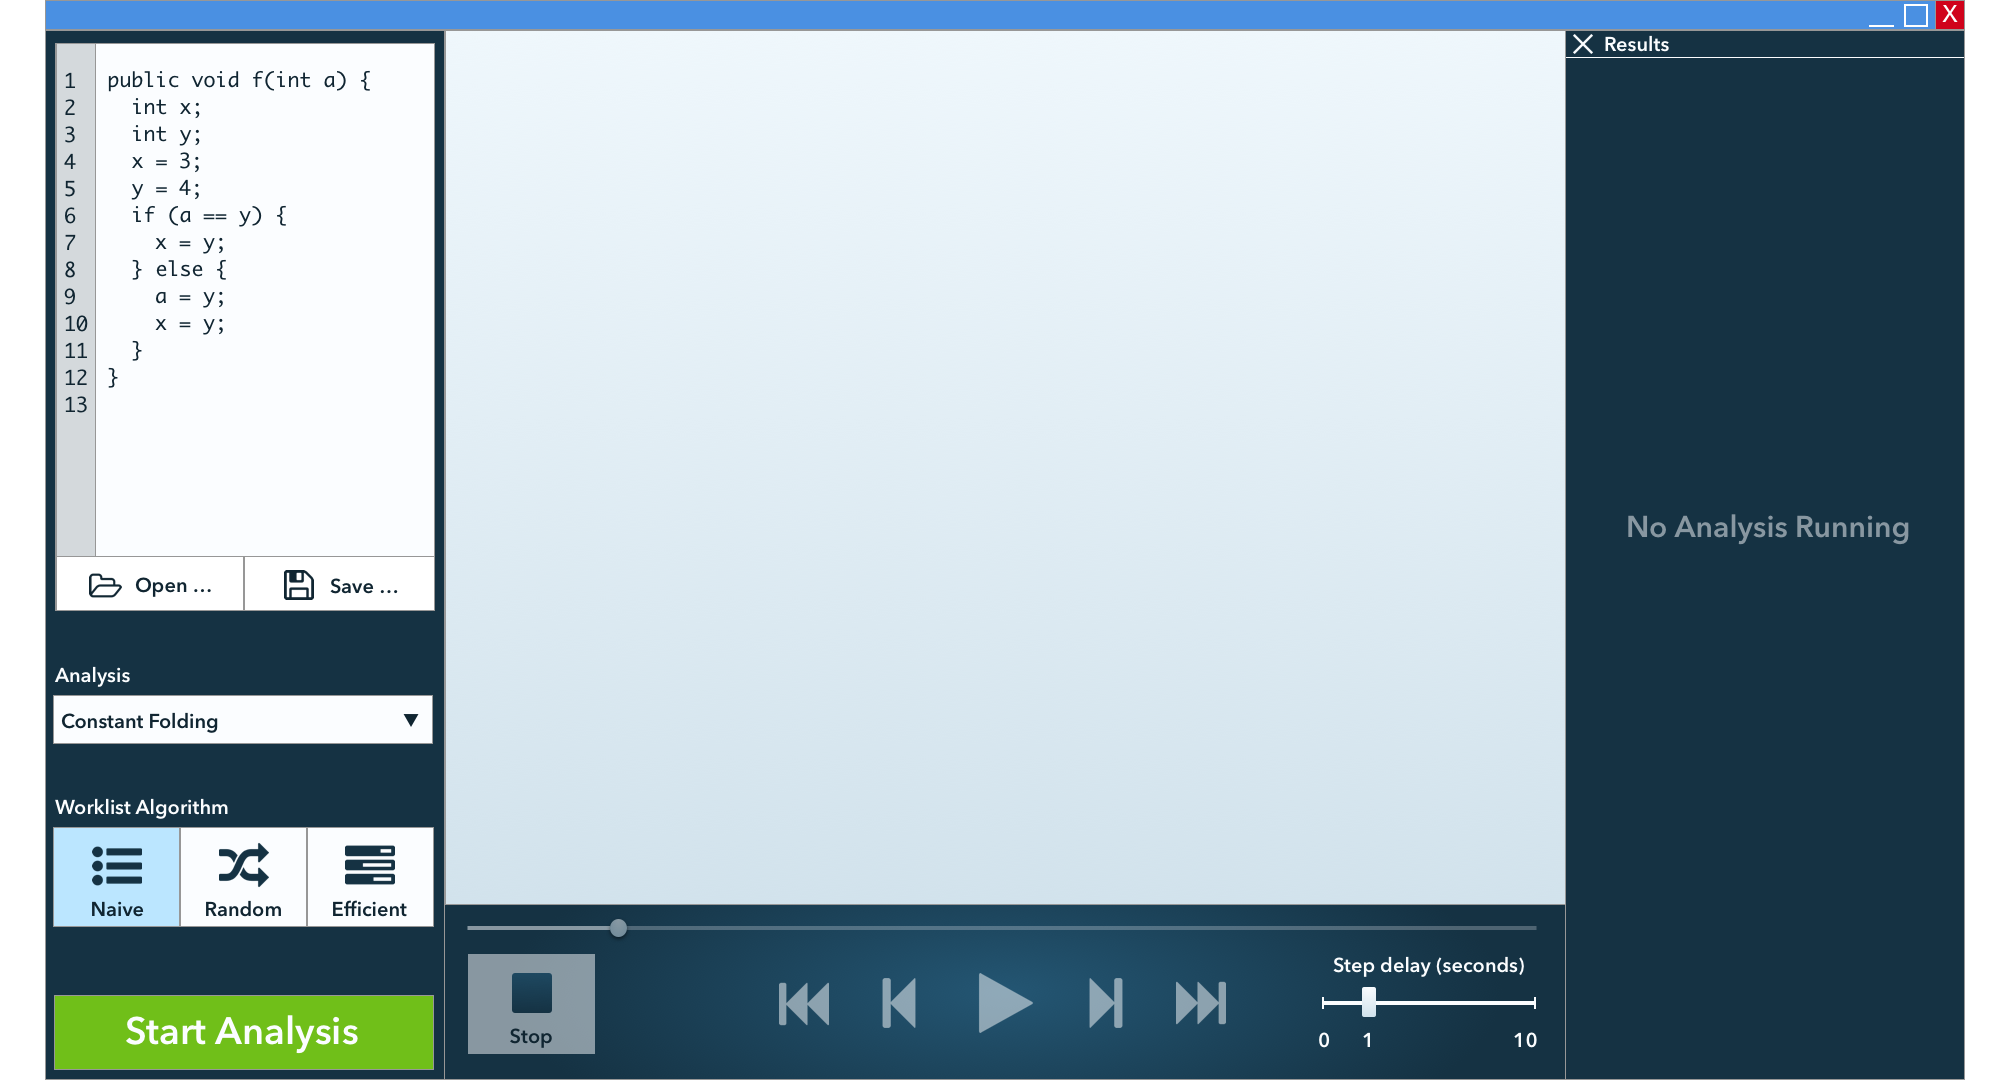
\includegraphics[angle=90, width=0.8\textwidth]{empty}
\end{figure}

\begin{figure}[H]
\caption{GUI während Ausführung der Analyse}
\centering
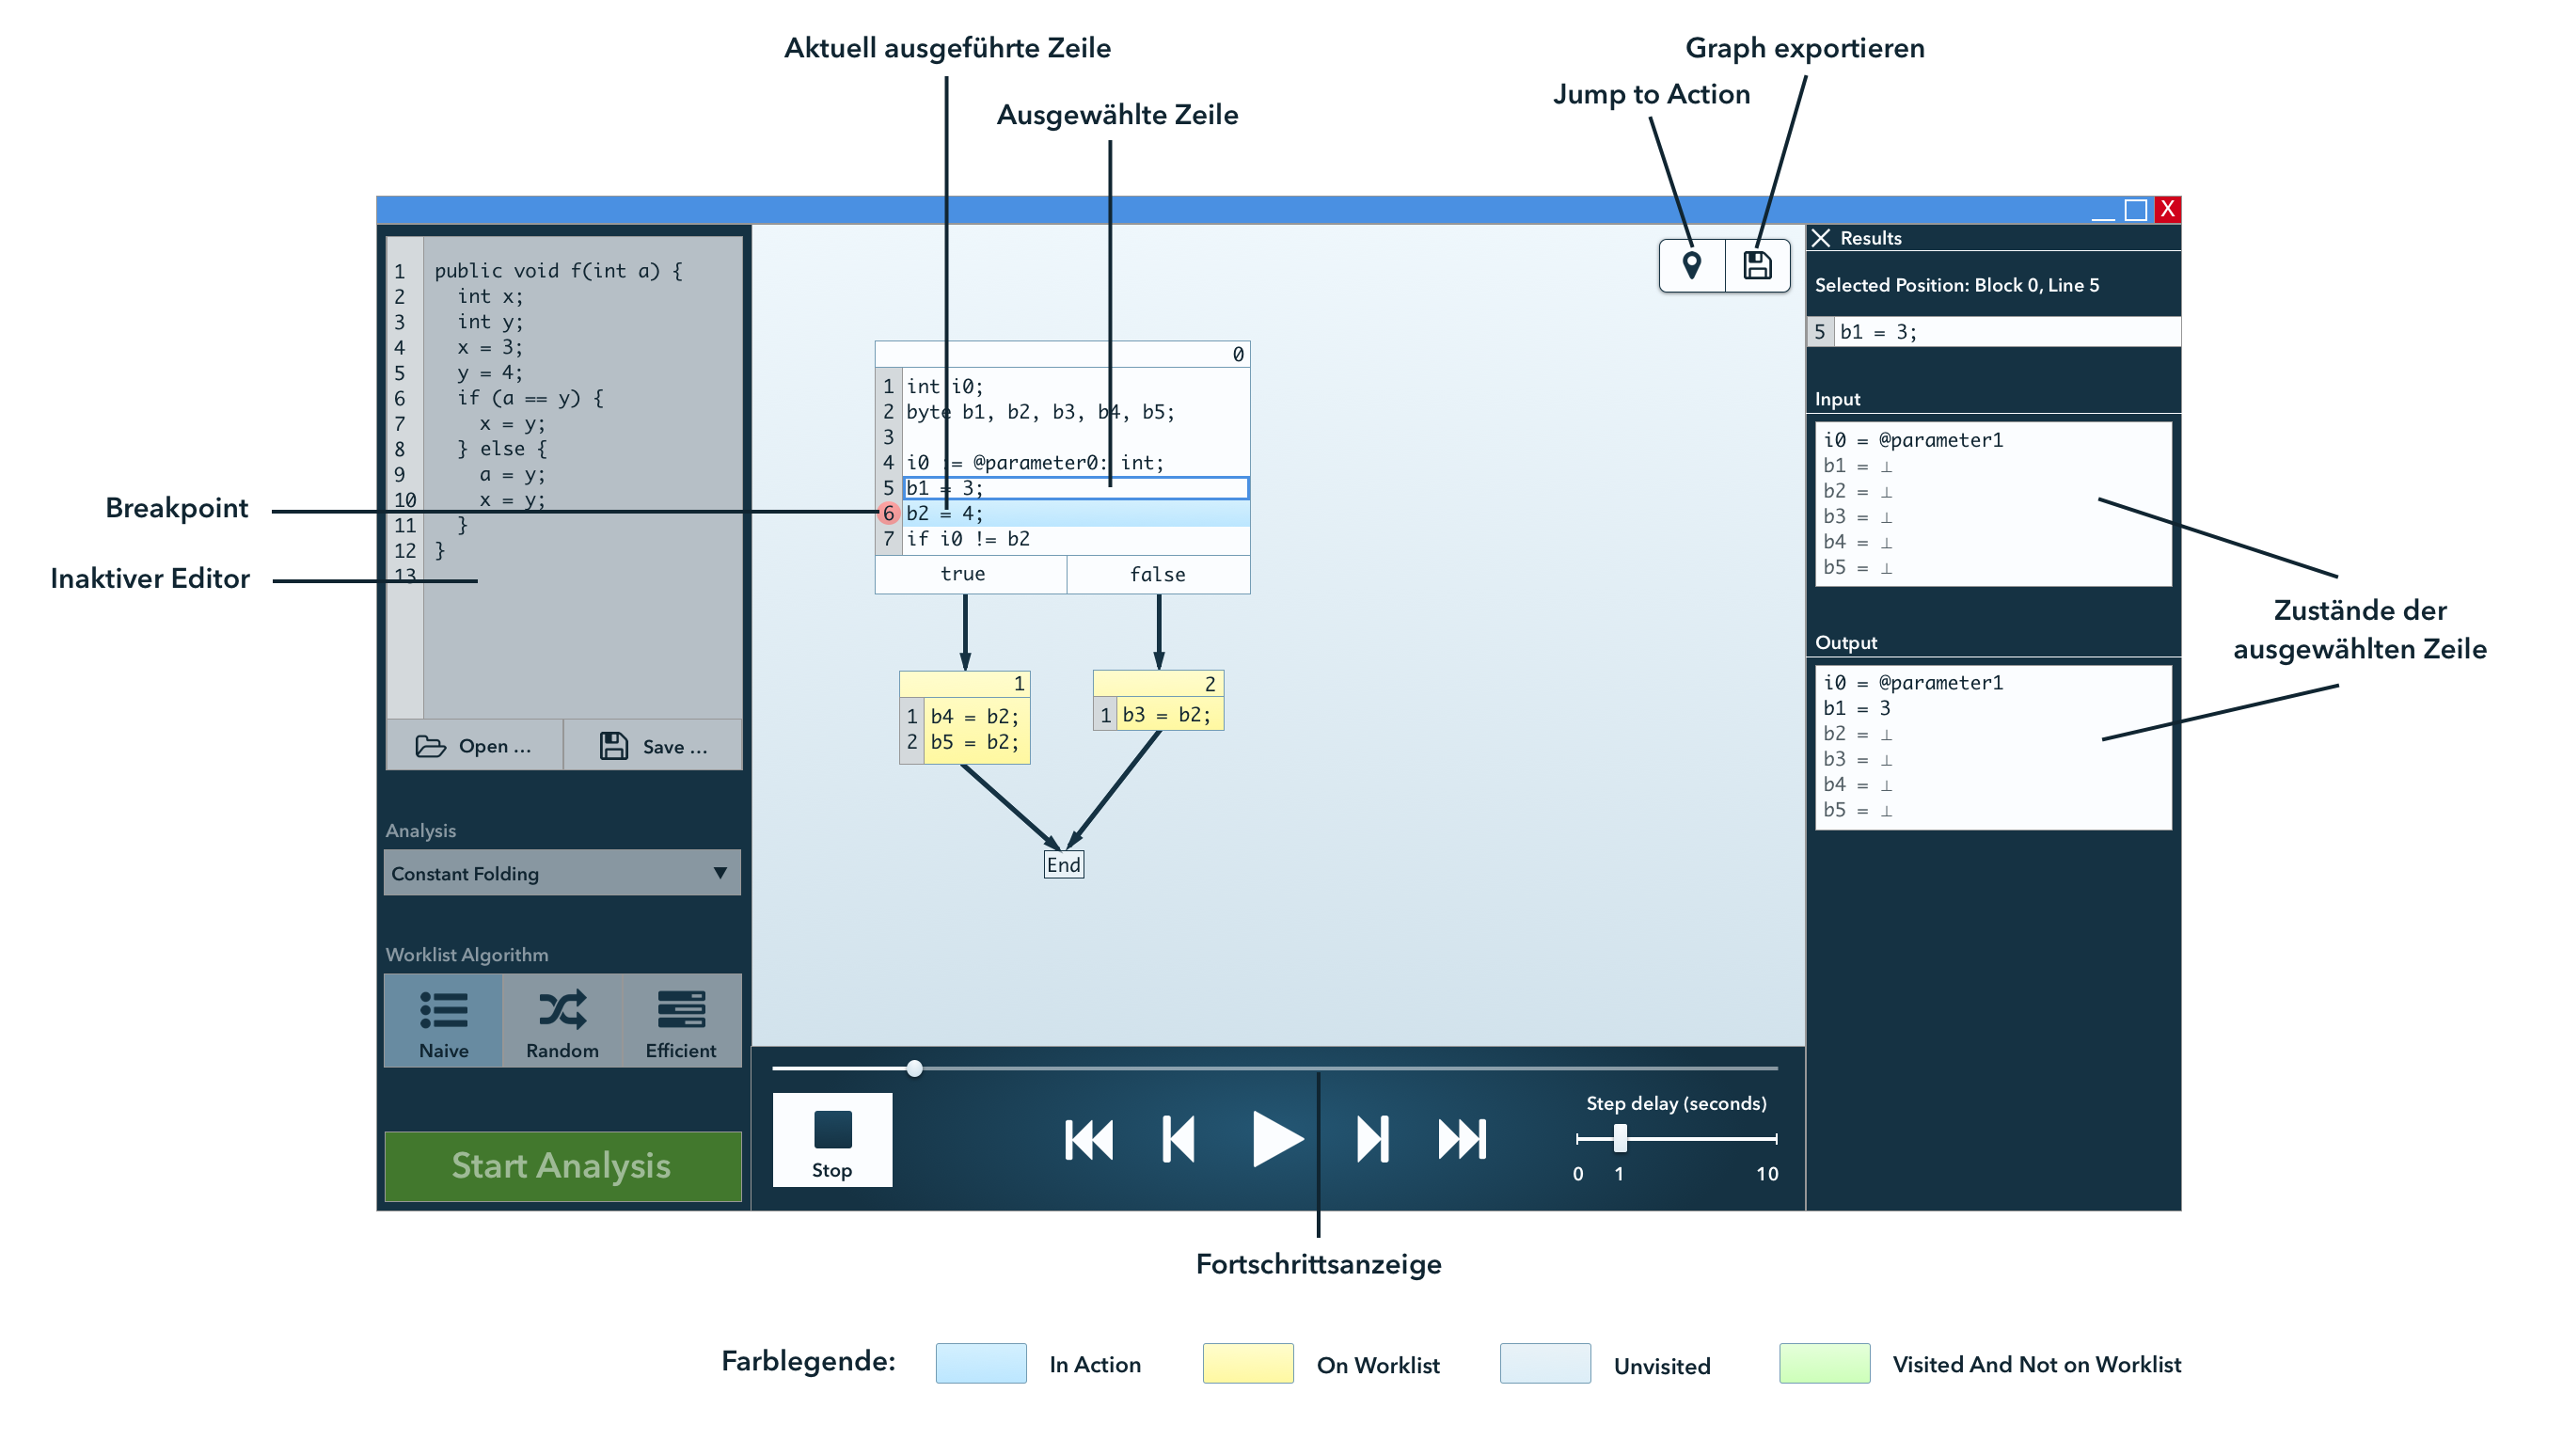
\includegraphics[angle=90, width=0.93\textwidth]{running}
\end{figure}
	
	% if you want to have the full glossary, not only the mentioned stuff
	% \glsaddall 
	
	\printglossaries
	
	
\end{document}